\documentclass[a4paper,titlepage,11pt,twoside,openright]{book}

\usepackage{lineno}
\linenumbers

%\setlength\textwidth{15cm}
\usepackage[margin=1.2in]{geometry}
% \usepackage{vmargin}
% \evensidemargin=3.5cm
% \oddsidemargin=4cm

\usepackage{graphicx}
\usepackage[square,numbers]{natbib} 
\usepackage[hidelinks]{hyperref}
\usepackage[utf8x]{inputenc}
\usepackage[italian,english]{babel}

\usepackage{amsmath}

\usepackage{multirow}
\usepackage[euler]{textgreek} % upright greek

\usepackage[usenames,dvipsnames]{xcolor}

% \evensidemargin=1.5cm
% \oddsidemargin=2.5cm

\setcounter{secnumdepth}{2}
\setcounter{tocdepth}{2}

%\captionsetup{font=small,labelfont={sf}}

%\input{mydefinitions.sty}

%% HEP stuff
\usepackage{hepunits}
\providecommand{\fbinv}{\ensuremath{\mathrm{\,fb}^{-1}\xspace}}
\providecommand{\pbinv}{\ensuremath{\mathrm{\,pb}^{-1}\xspace}}
\providecommand{\mgg}{\ensuremath{m_{\gamma\gamma}}\xspace}
\providecommand{\mee}{\ensuremath{m_{e^-e^+}}\xspace}
\providecommand{\phoIso}{\ensuremath{\mathrm{Iso}_\gamma}\xspace}
\providecommand{\chIso}{\ensuremath{\mathrm{Iso_{Ch}}}\xspace}
\providecommand{\trkIso}{\ensuremath{\mathrm{N_{Trk}}}\xspace}
\providecommand{\hoe}{\ensuremath{\mathrm{H/E}}\xspace}
\providecommand{\sieie}{\ensuremath{\sigma_{i\eta i\eta}}\xspace}
\providecommand{\sipip}{\ensuremath{\sigma_{i\phi i\phi}}\xspace}
\providecommand{\rnine}{\ensuremath{R_{9}}\xspace}
\providecommand{\Grav}{\PXXG\xspace}
\providecommand{\Ggg}{\ensuremath{\mathrm{\PXXG \rightarrow}\gamma\gamma}\xspace}
\providecommand{\Zee}{\ensuremath{\mathrm{Z \rightarrow}e^{+}e^{-}}\xspace}
\providecommand{\Zmmg}{\ensuremath{\mathrm{Z \rightarrow}\mu^{+}\mu^{-}\gamma}\xspace}
\providecommand{\pT}{\ensuremath{\mathrm{p_{T}}}\xspace}
\providecommand{\gaga}{\ensuremath{\gamma \gamma}\xspace}
\providecommand{\gj}{\ensuremath{\gamma j}\xspace}
\providecommand{\jj}{\ensuremath{jj}\xspace}

\providecommand{\fgaga}{\ensuremath{f_{\gamma \gamma}}\xspace}
\providecommand{\fgj}{\ensuremath{f_{\gamma j}}\xspace}
\providecommand{\fjj}{\ensuremath{f_{jj}}\xspace}

\providecommand{\pt}{\pT\xspace}
\providecommand{\mG}{\ensuremath{\mathrm{m_\Grav}}\xspace}
\providecommand{\scE}{\ensuremath{E_{SC}}\xspace}
\providecommand{\absScEta}{\ensuremath{|\eta_{SC}|}\xspace}
\providecommand{\DeltaR}{\ensuremath{\Delta\mathrm{R}}\xspace}
\providecommand{\DeltaEta}{\ensuremath{\Delta\eta}\xspace}
\providecommand{\expectZ}{\ensuremath{Z^{0}_{expect}}\xspace}
\providecommand{\Minuit}{{\textsc{minuit}}\xspace\xspace}
\providecommand{\RS}{{\textsc{RS}}\xspace\xspace}
\providecommand{\ADD}{{\textsc{ADD}}\xspace\xspace}
\providecommand{\CLs}{\ensuremath{\mathrm{CL_{s}}}\xspace}
\providecommand{\chisq}{\ensuremath{\chi^2}\xspace}

\providecommand{\lumisix}{\ensuremath{35.9\fbinv}\xspace}
\providecommand{\lumisixICHEP}{\ensuremath{12.9\fbinv}\xspace}
\providecommand{\lumifif}{\ensuremath{3.3\fbinv}\xspace}
\providecommand{\lumififBon}{\ensuremath{2.7\fbinv}\xspace}
\providecommand{\lumififBoff}{\ensuremath{0.6\fbinv}\xspace}

\providecommand{\mgg}{\ensuremath{m_{\gamma\gamma}}\xspace}
\providecommand{\phoIso}{\ensuremath{\mathrm{Iso}_\gamma}\xspace}
\providecommand{\chIso}{\ensuremath{\mathrm{Iso_{Ch}}}\xspace}
\providecommand{\hoe}{\ensuremath{\mathrm{H/E}}\xspace}
\providecommand{\sieie}{\ensuremath{\sigma_{i\eta i\eta}}\xspace}
\providecommand{\rnine}{\ensuremath{R_{9}}\xspace}
\providecommand{\Grav}{\PXXG\xspace}
\providecommand{\Ggg}{\ensuremath{\mathrm{\PXXG \rightarrow}\gamma\gamma}\xspace}
\providecommand{\Zee}{\ensuremath{\mathrm{Z \rightarrow}e^{+}e^{-}}\xspace}
\providecommand{\Hgg}{\ensuremath{\mathrm{Z \rightarrow}\gamma\gamma}\xspace}
\providecommand{\Zmmg}{\ensuremath{\mathrm{Z \rightarrow}\mu^{+}\mu^{-}\gamma}\xspace}
\providecommand{\pT}{\ensuremath{\mathrm{p_{T}}}\xspace}
\providecommand{\gaga}{\ensuremath{\gamma \gamma}\xspace}
\providecommand{\gj}{\ensuremath{\gamma j}\xspace}
\providecommand{\jj}{\ensuremath{jj}\xspace}

\providecommand{\fgaga}{\ensuremath{f_{\gamma \gamma}}\xspace}
\providecommand{\fgj}{\ensuremath{f_{\gamma j}}\xspace}
\providecommand{\fjj}{\ensuremath{f_{jj}}\xspace}

\providecommand{\pt}{\pT\xspace}
\providecommand{\mG}{\ensuremath{\mathrm{m_\Grav}}\xspace}
\providecommand{\scEta}{\ensuremath{\eta_{SC}}\xspace}
\providecommand{\DeltaR}{\ensuremath{\Delta\mathrm{R}}\xspace}
\providecommand{\DeltaEta}{\ensuremath{\Delta\eta}\xspace}
\providecommand{\expectZ}{\ensuremath{Z^{0}_{expect}}\xspace}
\providecommand{\Minuit}{{\textsc{minuit}}\xspace\xspace}
\providecommand{\RS}{{\textsc{RS}}\xspace\xspace}
\providecommand{\ADD}{{\textsc{ADD}}\xspace\xspace}
\providecommand{\CLs}{\ensuremath{\mathrm{CL_{s}}}\xspace}
\providecommand{\chisq}{\ensuremath{\chi^2}\xspace}

\providecommand{\pb}{\ensuremath{\mathrm{pb}\xspace}}
\providecommand{\fb}{\ensuremath{\mathrm{fb}\xspace}}

\providecommand{\PbWO}{PbWO\ensuremath{_4}\xspace}

\begin{document}

\clearpage\chapter*{Abstract}

Although the Standard model of particle physics (SM) describes with extreme success the
fundamental interaction of matter it does not provide a description for open question of
modern physics. The nature of cosmological dark matter, a quantum description of gravity and
the hierarchy problem cannot included in the framework of the SM.

For this reason several extension have been proposed throughout the year to address the open problems.
The beyond the standard model frameworks (BSM) often predicts the existence of additional particles,
either arising from additional symmetries introduced by the model or by the inclusion of gravity.
Some of the parameter space of these models can be covered by experiments at LHC, since the predicted particles
can have masses in the TeV range.

The diphoton resonant production is sensitive to spin-0 and spin-2 BSM resonances. These can be originated
by wrapped extra dimensions or extension of the Higgs sector which are typically included in BSM models.
The excellent energy resolution achieved with the CMS electromagnetic calorimeter (ECAL) and the clean signature
of the diphoton event makes this channel very attractive as a tool for the search of exotic resonances.
The sensitivity of the search in the diphoton channel is subordinated do the ECAL energy resolution and the
precision on the location of the interaction vertex. The search presented in this work has been conducted
on data collected by the CMS experiment at LHC with proton-proton collisions at a center-of-mass energy of 13 TeV,
for a total integrated luminosity of 35.9fb$^{-1}$).
No significant deviation from the standard model prediction has been highlighted by the analysis, thus
exclusion limits on the graviton production cross-section have been established in the context of the Randall-Sundrum
extra dimensions model.
The limits varies between 10~fb and 1~fb depending on the mass and coupling of the resonance in the 
$0.5 < m < 4$~TeV and $0.01 < \kappa < 0.2$ ranges.

The LHC program foresees an high luminosity phase starting from 2026 (HL-LHC), during which the
instantaneous luminosity will reach the record value of $7.5\times10^{34}\mbox{cm}^{-2}\mbox{s}^{-1}$, five times
the current one. On one hand higher instantaneous luminosity will bring benefits to the physics analysis by providing
a dataset 10 times larger than what will be available during the LHC phase but, on the other hand will post severe
challenges to the event reconstruction given the high number of overlapping collisions.
CMS is already planning various actions and detector upgrades to match the physics goal of HL-LHC.
Among those the introduction of time into the event reconstruction will require the installation of
a completely new detector. Technologies suitable for the measurement of charged particles time with a precision
of 30~ps have been identified through a series of test with particles beam. In the same tests the intrinsic time
resolution of the ECAL has been proved to be better than 20~ps for energetic electrons and photons.
The R\&D campaign has been coupled to simulation studies to quantify the expected gain in performance provided 
by a time-aware event reconstruction. The simulation studies show a general improvement for observable of interest for
the HL-LHC physics program.


\tableofcontents

\mainmatter

\clearpage\chapter{Introduction}
\label{chapter:introduction}

This thesis revolves around measurements involving a two photon final state.
The diphoton decay channel has been one of the two decay modes that led to the
first observation of the Higgs boson~\cite{cms_atlas_hgg_comb}. The same
final state provide a probe to test models describing new physics such as quantum gravity
effective theories based on extra dimensions or Super Symmetry (SUSY) models with an extended
Higgs sector. The nature of the photon restrict the
particles that can decay to a two photon system to bosons with either
spin equal to zero or spin strictly greater than one~\cite{landau,yang}.
A search for beyond the standard model (BSM) resonances, performed with p-p collision data collected by the CMS experiment,
is presented in Chapter~\ref{chapter:diphoton} together with the description of the calibration procedure (Chapter~\ref{chapter:ecal}
of the detector component that contributes the most to the detection of photons in CMS (i.e. the electromagnetic calorimeter).

Measurement involving a diphoton system in the final state also includes the measurement of the Higgs boson self coupling
through di-Higgs production in p-p collisions. This standard model process is extremely rare, thus its observation is
only possible with a large dataset of p-p collisions. Such dataset will be produced during the high luminosity
phase of LHC (HL-LHC), in Chapter~\ref{chapter:upgrade} the major goal and challenges of are described together with
the preliminary studies to incorporate the time information into the event reconstruction of CMS as a way to meet
the performance needed to fully exploit data collected in the high luminosity phase.

In the following sections the theoretical framework of fundamental interaction is briefly introduced.
The main focus is describe the standard model, the phenomenology of hadronic collisions and the models
which gives rise to a BSM resonant diphoton production.

\section{The standard model of particle physics}
During the 20th century the development of new technologies enabled experimental
physicist to explore matter at the atomic and sub-atomic levels. At these levels
is possible to explore the building blocks of matter and the interactions between them.

A theory has been constructed during the past century which describes and predicts
a large part of the natural processes that are know today. The Standard Model of particle physics (SM)
describes in coherent way three types of interactions between sub-atomic particles:
the behavior of electromagnetic, weak and strong interaction at a quantum level is
addressed by the SM, this in fact allows us to describe a variety of phenomena with a
single mathematical framework.

The SM is build upon relativistic quantum field theory. The constituents of matter are particles
with half-integer spin that follow the Fermi-Dirac statistic while the interactions are mediated by
integer spin particles which follow Bose-Einstein statistic. Is common to refer at the first group as
fermions and to the second as bosons. Tables \ref{tab:fermions} and \ref{tab:bosons}
show the fermions and bosons described by the SM and their
main properties. 

\begin{table}[ht]
  \begin{center}
    \begin{tabular}{|c|cc|cc|cc|c|c|}
    \hline
    & \multicolumn{2}{c|}{$1^{\textnormal{st}}$ gen.}
    & \multicolumn{2}{c|}{$2^{\textnormal{nd}}$ gen.}
      & \multicolumn{2}{c|}{$3^{\textnormal{rd}}$ gen.}
      & $Q$
      & Colour Charge \\
    \hline
    \hline
    \multirow{2}{*}{leptons} &
    \textnu$_{\textnormal{e}}$            & \small{$\sim 0$} &
    \textnu$_{\textnormal{\textmugreek}}$ & \small{$\sim 0$} &
    \textnu$_{\textnormal{\texttau}}$     & \small{$\sim 0$} &
    0 & 0 \\
    &
    e            & \small{$511 \mathrm{keV}/\mathrm{c}^2$}   &
    \textmugreek & \small{$105.7 \mathrm{MeV}/\mathrm{c}^2$} &
    \texttau     & \small{$1.777 \mathrm{GeV}/\mathrm{c}^2$} &
    -1 & 0 \\
    \hline
    \multirow{2}{*}{quarks} &
    u & \small{$1.7-3.1\mathrm{MeV}/\mathrm{c}^2$}         &
    c & \small{$1.29^{+0.05}_{-0.11}\mathrm{GeV}/\mathrm{c}^2$}  &
    t & \small{$172.9^{+1.1}_{-1.1}\mathrm{GeV}/\mathrm{c}^2$} &
    2/3 & $r,g,b$ \\
    &
    d & \small{$4.1-5.7\mathrm{MeV}/\mathrm{c}^2$} &
    s & \small{$100^{+30}_{-20}\mathrm{MeV}/\mathrm{c}^2$} &
    b & \small{$4.19^{+0.18}_{-0.06}\mathrm{GeV}/\mathrm{c}^2$} &
    -1/3 & $r,g,b$  \\
    \hline
    \end{tabular}
  \end{center}
  \caption{Spin-$\tfrac{1}{2}$ fermions masses, electric charges (in units of the positron charge) and color charges~\cite{PDG}.}
  \label{tab:fermions}
\end{table}

\begin{table}[ht]
  \begin{center}
    \begin{tabular}{|c|c|c|c|}
    \hline
    & Mass (GeV)
    & $Q$
    & Colour Charge \\
    \hline
      \hline
      Photon ($\gamma$) & 0 & 0 & 0 \\
      Gluon ($g$) & 0 & 0 & $r,g,b$ \\
      W & $80.385 \pm 0.015$ & $\pm 1$ & 0 \\
      Z$^0$ & $91.188 \pm 0.002$ & 0 & 0 \\
    \hline
    \end{tabular}
  \end{center}
  \caption{Spin-1 bosons masses and charges~\cite{PDG}.}
  \label{tab:bosons}
\end{table}

Fermions differ from each other by mass and coupling to the force carriers, a charge is associated
to each interaction so a total of four values is used to identify a fermion: three charges and one mass.
Fermions with non-null color charge are named quarks and interact strongly with each other through the exchange
of gluons, the strong force carriers. The other fermions, called leptons, that are insensitive to
the strong force interacts only electroweakly.

At the core of the SM there is the concept of gauge invariance.
Since Maxwell's unification of electric and magnetic interactions, gauge invariance
has played a strategic role in the description of the fundamental interaction of matter.
The requirement of a symmetry in the Lagrangian of a theory accounts for conservation of
charges, via the Noether's theorem.
The mediators of the interaction are introduced to preserve the conservation of
the free particle Lagrangian under the gauge transformation of the type $\psi \to e^{i\alpha}\psi$, where
$\psi$ is a generic fermion field.

In these terms the SM is based on a group of three symmetries $SU_C(3)\times SU_L(2) \times U_Y(1)$.
The three symmetries are related to three local gauge invariances of the Lagrangian that describes the interaction
between the particles described above.

$SU_C(3)$ is related to the strong interaction mediated by the massless gluons. It conserves the colour charge
carried by quark and gluons which appear as colour triplets under $SU_C(3)$ transformation.
The experimental evidence is that coloured particles cannot propagate freely.
Quarks and gluons are only observed in bound states as mesons $q\bar{q}$ and barions $qqq$.
This behaviour is known as
asymptotic free, i.e. he coupling is asymptotically weaker as energy increases and distance decreases
and conversely it becomes stronger at larger distances.

The $SU(2)_{L} \times U(1)_{Y}$ group is associated to electroweak interactions, which are the
unified description of electromagnetism and weak interactions. The long-range electromagnetic
interaction is mediated by the massless photon ($A_{\mu}$ field), while the short-range weak force carriers are the
massive $W^{+}$, $W^{-}$ and $Z^{0}$ bosons. Unlike the gluons the electroweak mediators
are not the direct fields introduced to preserve the gauge invariance but instead are combinations
of them. In particular the $W_{\mu}^3$ and $B_{\mu}$ introduced respectively for the $SU_L(2)$ and $U_Y(1)$ symmetries
are mixed to obtain the physical $A_{\mu}$ and $Z_{\mu}$ fields:
\[
\begin{split}
  W_{\mu}^{\pm} & = \frac{1}{\sqrt{2}}\left(W_{\mu}^{1}\mp i W_{\mu}^{2}\right) \\
  \left(
  \begin{array}{c}
  A_{\mu} \\ Z_{\mu}
  \end{array}
  \right)
  & =
  \left(
  \begin{array}{cc}
  \cos\theta_{W} & \sin\theta_{W} \\
  -\sin\theta_{W} & \cos\theta_{W}
  \end{array}
  \right)
  \left(
  \begin{array}{c}
  B_{\mu} \\ W_{\mu}^{3}
  \end{array}
  \right) \quad ,
\end{split}
\]

where Weinberg mixing angle ($\theta_W$) has been measured at the Z-pole at LEP as
$sin^2(\theta_W) = 0.23153 \pm 0.00016$.

The mixing is also reflected in the conserved charges for which the following relation holds:
\[
  Q = T_3 + \frac{Y}{2}
\]
where $Q$ is the electric charge, $Y$ the $U_Y(1)$ hypercharge and $T_3$ is the third component of the weak
isospin $T$ conserved by the $SU_L(2)$ symmetry.

The $W^{\pm}$ bosons couple only to the left-handed components $\psi_{L}$ of the fermion fields,
while the $Z^{0}$ and $\gamma$ bosons couple to both $\psi_L$ and
$\psi_R$, thus leading to the observed parity-violation phenomena of weak interactions.
The asymmetry between right and left handed fermions also forbids the inclusion of a
Yukawa mass terms into the standard model Lagrangian since such a term would not be invariant under $SU_L(2)$
transformation.
This fact has an remarkable consequence: the three generation of leptons and quarks summarized
in Table~\ref{tab:fermions} are identical from the perspective of the strong and electroweak interactions
since they only differ for their masses.
Table~\ref{tab:charges} summarize the charges for all known fermions families: 
\begin{table}[ht]
  \begin{center}
    \begin{tabular}{|c|c|c|c|c||c|c|c|c|c|}
      \hline
      & $T$
      & $T_3$
      & $Y$
      & $Q$
        &
      & $T$
      & $T_3$
      & $Y$
      & $Q$ \\
          \hline 
      $l_L$ & $1/2$ & $-1/2$ & $-1$ & $-1$  & $q_L^{down}$ & $1/2$ & $-1/2$ & $1/3$ & $-1/3$ \\      
      $\nu_L^l$ & $1/2$ & $1/2$ & $-1$ & $0$  & $q_L^{up}$ & $1/2$ & $1/2$ & $1/3$ & $2/3$ \\
      $l_R$ & $0$ & $0$ & $-2$ & $-1$  & $q_R^{down}$ & $0$ & $0$ & $4/3$ & $2/3$ \\
      $\nu_R^l$ & $0$ & $0$ & $0$ & $0$  & $q_R^{up}$ & $0$ & $0$ & $-2/3$ & $-1/3$ \\
      \hline
    \end{tabular}
  \end{center}
  \caption{Charges (quantum numbers) of leptons (left) quarks (right).}
  \label{tab:charges}
\end{table}

Notably the right-handed neutrino is sterile in the standard model, i.e. it does not couple to
any of the three forces carriers. 

Bosons and fermions in the theory outlined above are all massless, this is in evident contradiction with
the observation of masses that vary across several other of magnitude from the almost massless neutrinos
to the heaviest quark.
The spontaneous electroweak symmetry breaking mechanism (EWSB) of a local gauge
symmetry was proposed by Englert, Brout~\cite{37}, Higgs~\cite{higgs} and others and it
is shortly outlined in the following. It can be applied to any renormalizable quantum field theory,
such as the standard models. The mass
of the gauge bosons can be generated by a scalar field. The chosen doublet of complex
scalar fields ($SU_L(2)$) is of the form:
\[
  \phi = \frac{1}{\sqrt{2}}\begin{bmatrix}
    \sqrt{2}\phi^+ \\
    \phi^0 + ia^0
  \end{bmatrix}
\]
with $\phi^0$ and $a^0$ being the CP-even and CP-odd neutral components, and $\phi^+$ being the
complex charged component of the Higgs doublet. The standard model Lagrangian is extended with
to include the so-called Higgs scalar potential:
\[
  V(\phi) = \mu^2\phi^{\dagger}\phi + \frac{\lambda}{2}(\phi^{\dagger}\phi)^2
\]
with the real parameter $\mu^2$ and quartic coupling $\lambda$, the Higgs self-coupling parameter.
The electroweak symmetry is then said to be spontaneously broken as the SM Lagrangian
stays invariant under the symmetry, but the ground state $<\phi> = \frac{1}{\sqrt{2}}\begin{bmatrix}0 \\ \nu \end{bmatrix}$
of the Higgs potential does not.
With $\nu = \frac{\sqrt{2}|\mu|}{\lambda}$ being the vacuum expectation value, its value has been
measured experimentally at LHC and is 246 GeV [8].
Gauge boson acquire mass through the spontaneous symmetry breaking mechanism while for fermions
the mass derives from Yukawa interaction with the Higgs scalar field.
The mass of the Higgs boson is a free parameter of the theory and was measured experimentally by ATLAS and CMS to be
$m_H = \lambda\cdot\nu = 125.01\pm 0.21(stat) \pm 0.11 (syst)$ GeV [8].
Till now all the measured properties (spin and couplings) do not show any significant discrepancy with
the standard model prediction.

The standard model described above has proven over the years to be remarkably accurate in describing and
predicting the interaction of matter at the quantum level.
However there a number of processes observed in Nature that cannot be explained by the otherwise complete model:
\begin{itemize}
\item Cosmological dark matter.
\item Matter-antimatter asymmetry.
\item Neutrinos oscillations and masses.
\end{itemize}
To name some of them. Furthermore the SM lacks a quantum description of gravity and also requires
a ``fine tuning'' (more later) of some of its parameters.

These issue are addressed by several models extending the SM, most of them predicts the existence of new particles
(arising from the same gauge invariance request explained above) that could be observed either through the
products of their decay or from virtual interference with standard model interactions.
In both cases hadronic collision offers a unique way to test such models providing both the possibility
to produce them or infer their existence from precise measurement of the standard model parameters.

\section{Proton-proton collisions}
The precise measurement of the electroweak sector at the LEP and SLC electron-positron colliders and the discovery of the top
quark at Tevatron proton-antiproton collider, the yet to be observed Higgs boson and the search for BSM physics led
to the construction of the Large Hadron Collider (LHC).

Hadronic colliders, in the context of high energy physics, are great tools for discoveries since
protons are composite particles and thus both the hard scattering energy and its nature are not restricted by
the machine parameters but covers a wide range of possibilities.
The inner structure of the proton have been extensively studied in recent years at the electron-proton collider HERA
at DESY~\cite{hera}. The proton, as all other barions, is made of three ``valence'' quark surrounded by a ``sea''
of gluons and quark-antiquark pairs. Quarks and gluons in this context are referred to as partons. 
This qualitatively description is translated into a quantitative description by the DGLAP equations using perturbative
quantum chromodinamics (QCD)~\cite{altarelli_parisi,gribov,dokshitzer}.
The probability to find a parton carrying a fraction ``$x$'' of the total proton momentum
is described by the parton density functions (PDFs).
As shown in Figure~\ref{fig:pdfs} the valence quark dominates over the sea partons for $x>0.1$.
The PDFs depends on the momentum transferred in the scattering process, in particular for
larger values of momentum transfer $\mu^2$ the gluon PDFs dominates over the valence quark. For this reason
``gluon-fusion'' initiated processes dominates at LHC.

\begin{figure}
  \centering
  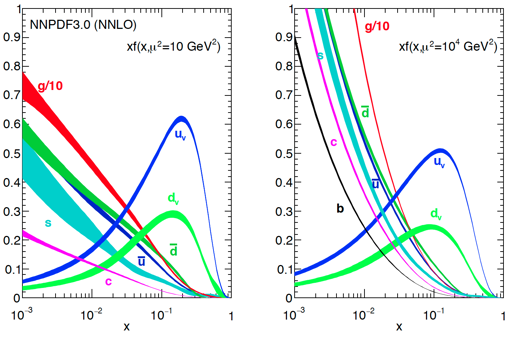
\includegraphics[width = 0.7\textwidth]{figures/introduction/pdfs.png}
  \caption{
    Distributions of $x$-times the unpolarized parton distribution function $f(x)$
    obtained in the NNPDF 3.0 global analysis at the scales of $\mu^2 = 10 \mathrm{GeV}^2$ (left) and
    $10^4 \mathrm{GeV}^2$ (right) at $\alpha_s(M_Z) = 0.118$~\cite{pdfs}.}
  \label{fig:pdfs}
\end{figure}

the perturbative QCD well describes the hard part of the hadronic collisions and the emission of
energetic quark and gluons as initial and final state radiation,
while the description of the formation of bounded QCD states from bare quark and gluons involves non-perturbative, low $\mu^2$
processes generally called ``hadronization''. 

The hadronization of quark and gluons coming from high $\mu^2$ processes (hard scattering) gives rise
to a jet of collimated hadrons , which are usually reconstructed in collider experiments as energy clusters.
The kinematic of a jet is directly linked to the one of the original quark or gluon, allowing the reconstruction
of the hard scattering.

An hard scattering usually only involves a parton from each colliding proton, the other partons interact at low $\mu^2$
(soft interactions) giving rise to the so called ``underlying event'' i.e. particles of low transverse momentum $p_T$
produced in conjunction with the boosted products of the hard interaction.

\section{Extra dimensions and the hierarchy problem}
The hierarchy problem is a common way to, within the high energy physics community, refer to the large
discrepancy arising between the effective value of a constant and the fundamental value it has
in the Lagrangian that describes the dynamics of the model under consideration

An example in SM is given by higher order corrections to the Higgs boson mass. These includes loops of
massive particles which for one fermion give a correction expressed as:
\[
  \Delta M_H^2 = \frac{\lambda_f^3}{4\pi}(\Lambda^2 + m_H^2)
\]
If one imposes a cutoff at a scale $\Lambda$ close to the Planck mass ($M_{Pl}\sim 10^{19}$GeV) a cancellation
of the radiative correction for this fermion loops occurs for $m_H = 246$GeV and $(m_H/Lambda)^2 \sim 10^{34}$
(here $m_H$ the fundamental Higgs boson mass equal to the vacuum expectation value for the Higgs field and
$\Delta M_H$ represent the correction that gives the observed Higgs boson mass).

Is evident that such a small value of $(m_H/Lambda)^2$ represent a ``fine-tuning'' of the theory which otherwise
would give rise to an incredibly huge Higgs boson mass (compared to all other particles in the standard model).
The ``fine-tuning'' cannot be explained within the framework of the SM alone,
however extra dimension models offer a solution to this fine tuning.

Extra dimension models (ED) were introduced by Kaluza-Klein~\cite{kk} in attempt to unify the electromagnetism
with the description of gravity given by Einstein's general relativity.
The general idea is that existence of a multidimensional space-time with at least 4 space dimensions
and one time dimension. This space-time is an extension of the four-dimensional Minkowsky space and the weakness of
the gravity interaction is explained by its propagation through the extra dimensions.

Extra dimension as solution for the hierarchy problems were first proposed
by Arkani, Dimopoulos and Dvali (thus the name ADD model)~\cite{ADD}.
The existence of $n$ additional spatial dimensions, compactified with
average radius $R$, produces an effective Planck mass in our four-dimensional world that is related to the true
Planck Mass by: $M_{Pl}^2 \sim M_{Pl(4_n)}^{n+2}R^n$. It is therefore possible, with appropriate values for $n$
and $R$, that the true value of the Planck scale ($M_{Pl(4_n)}$) could be on the order of the electroweak scale,
thus solving the SM hierarchy problem, while still producing the much larger apparent Planck
scale that we observe in our four-dimensional world.

Randall and Sundrum (RS) proposed an alternative model~\cite{RS}, with just one additional dimension
that has a warped geometry, described by curvature parameter $k$. The extra dimension $y$
is wrapped, meaning that it is curled up to a circle with a finite radius $r_c$ and curvature parameter $k$.
The five-dimensional space-time metric is given by:
\begin{equation}
  ds^2 = e^{-2ky}\eta_{\mu\nu}dx^{\mu}dx^{\nu} + d^2y 
\end{equation}
\label{eq:extra_dim_metric}

Imposing the boundary conditions of $y = 0$ and $|y| = \pi r_c = L$.
The two boundary conditions determine the warp factor of Equation~\ref{eq:extra_dim_metric}:
\[
  \frac{e^{-k|y(L)|}}{e^{-k|y(0)|}} = e^{-2kr_c}
\]
The RS model in contrast to ADD one only requires one extra dimension with $r_c \sim 15$ to solve the
hierarchy problem thanks to the wrapped geometry of the extra dimension.

\section{Extra dimension signatures in proton-proton collisions}
In both the ADD and RS models the perturbative KK expansion of the five-dimensional metric
gives origin to an infinite number of four-dimensional spin-2 fields (gravitons). Together with
the massless spin-2 boson associated to gravity an infinite number of massive gravitons are predicted to exist
at masses that are of the order of the TeV.
In the ADD model the four-dimensional massive states
are closely spaced and thus produce a degenerate spectrum when they decay into SM particles.
RS model instead predicts the existence of well separated mass states of which only the first one has a mass
within the energy reach of LHC.

The RS-like models can be further categorized depending on how much the SM fields propagates into the five-dimensional
space-time. In the ``bulk'' scenario the SM fields propagates in the five-dimensional space as the graviton field does
and while in the RS1 they are confined to the four-dimensional world.
In the bulk scenario the gravitons coupling to SM particles is proportional to the mass of the SM particle, for this
reason the primary search channel are final states with two gauge of Higgs bosons (Figure~\ref{fig:rs_coup}, left).
In the RS1 scenario instead the highest graviton decay branching ratio is in a photon pair (Figure~\ref{fig:rs_coup}, right).
The search described in Chapter~\ref{chapter:diphoton} thus focus on the RS1 model graviton.
\begin{figure}[ht!]
  \centering
  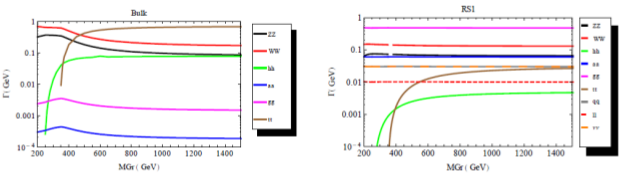
\includegraphics[width = 1.\textwidth]{figures/introduction/rs_coup.png}
  \caption{
    KK graviton branching fractions. Left: Bulk scenario. Right RS1 scenario.
    The dashed line represents the individual KK graviton decay rates to a pair of
    light fermions $f\bar{f}$.}
  \label{fig:rs_coup}
\end{figure}

Several searches have been performed at collider experiments searching for both ADD and RS like graviton
production. At Tevatron the CDF and D0 experiment graviton masses up to 500 GeV\cite{cdf_dipho, d0_dipho}.
The $95\%$ exclusion limits reach was extended to the TeV range by ATLAS and CMS already with data from 8 TeV LHC
collisions~\cite{atlas_dipho_2012, cms_dipho_2012_1}.

The diphoton final state is also sensitive to spin-0 resonances such as those predicted by SUSY models. SUSY models
introduce an additional symmetry to explain the large mass differences observed between SM particle, this leads
to the prediction of the existence to a partner to each of the known SM particles and also to an extend Higgs sector.
A popular model is the so called two-Higgs-Doublet-Model (2HDM)~\cite{spin0_1,spin0_2}, this was chosen as benchmark as
spin-0 signal in the search for diphoton resonances.

\section{Standard model diphoton production}
\label{sec:sm_dipho_prod}
The main background for the search of BSM resonances decaying to two photons is the standard model production
of photon pairs. Photon pairs production is possible through leading order processes involving two
initial state quarks $q\bar{q}\to\gamma\gamma$ (Figure~\ref{fig:lo_dipho}. Higher order terms in perturbative QCD also contribute to
the total production cross section as well as final state quark fragmentation,
the corresponding Feynman diagrams are illustrated in Figure~\ref{fig:lo_dipho}.
Given the importance of gluon initiated processes at LHC the ``box'' diagram diphoton production through gluon-fusion
also has a large contribution in the SM diphoton production.

\begin{figure}[hb]
  \centering
  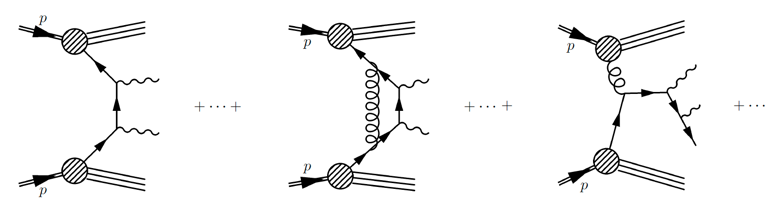
\includegraphics[width = 0.7\textwidth]{figures/introduction/lo.png}
  \caption{
    Feynman diagrams of the diphoton production processes, with the LO Born
    process $q\bar{q}\to\gamma\gamma$ (left), and the NLO contributions $q\bar{q}\to\gamma\gamma g$ (middle) and
    $q\bar{q}\to\gamma\gamma q$ (right) [61] and associated virtual corrections~\cite{61}.
  }
  \label{fig:lo_dipho}
\end{figure}

\begin{figure}[hb]
  \centering
  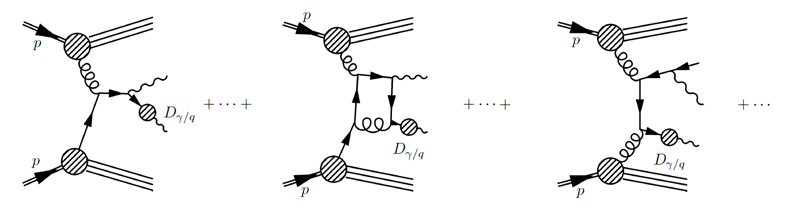
\includegraphics[width = 0.7\textwidth]{figures/introduction/nlo.png}
  \caption{
    Examples of diphoton production processes with one photon being produced via quark fragmentation~\cite{61}
  }
  \label{fig:nlo_dipho}
\end{figure}

\begin{figure}[hb]
  \centering
  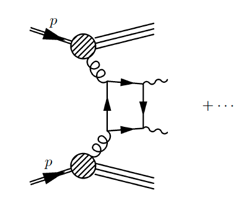
\includegraphics[width = 0.3\textwidth]{figures/introduction/box.png}
  \caption{
    Feynman diagram of the NNLO ’Box’ diphoton production process~\cite{61}.
  }
  \label{fig:lo_dipho}
\end{figure}


\clearpage\chapter{The LHC complex and the CMS experiment}
\label{chapter:cms}

In this Chapter a brief description of the Large Hadron Collider and of the CMS detector are
presented in order to contextualize the physics analyses that are described in the following chapters.
In particular, the CMS subdectors are described, since they are fundamental for the reconstruction of particles,
such as photons and products of partons hadronization.

\section{The Large Hadron Collider}

The Large Hadron Collider (LHC) is the largest and most energetic machine ever build to study
matter at the subatomic scale. It is operated by CERN and is located at the boarder between France and
Switzerland close to Geneve. It collides protons up to a center of mass energy of 13 TeV.

The LHC is located underground ($\sim 100$ m below the surface) and has a total lenght of about 27 km.
The tunnel that houses the LHC was previously occupied by the Large proton electron collider (LEP) that
played a crucial role in investigating the properties of the Z and W bosons.

The primary goal of LHC has been to study the electroweak simmetry breaking through first discovery of the Higgs boson and later
precision measurements of the its properties.
The energies explored by the collisions at LHC allow to probe the standard model up to scales of few TeV where
interactions not described by the SM could be observed in various production and decay processes.

The same machine is also used to accelarate and collide proton with ions or ions with ions.

The design of the LHC aims to reach a center of mass energy of 14 TeV and an istantaneous luminosity ($\mathcal{L}$)
of $10^{34}cm^{-2}s^{-1}$ for $p-p$ collisions. The scientific program span several decades, in the current phase it will
deliver to the experiments about $300 \fbinv$ of integrated luminosity, while it will reach $3000 \fbinv$ during the dacade
starting in 2025 (Figure~\ref{fig:lhc_plan}). 

\begin{figure}[!h]
  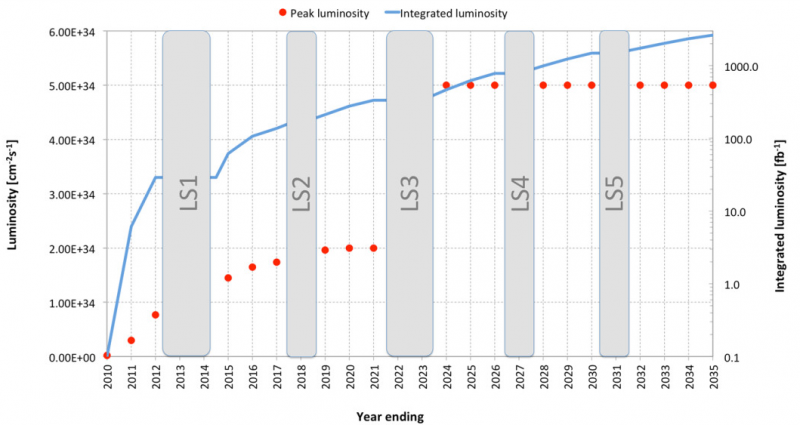
\includegraphics[width = 1.\textwidth]{figures/cms/Projected_LHC_Performance.png}
  \caption{Illustration of the foreseen LHC schedule, the current phase ends with long shutdown 3 (LS3). The high
    luminosity phase (HL-LHC) starts after LS3 and will last for a decade. LHC standard operation includes running
    periods during spring, summer and fall and a technical stop for small upgrades and mantainance during winter.
    Larger upgrades are carried out during long shutdowns (LS), a major one will be the upgrade of the LHC and of
  the experiments during LS3.}
  \label{fig:lhc_plan}  
\end{figure}

\section{LHC properties}
The high beam intensities necessary for reaching the design luminosity make the
use of two separate proton beams necessary. The collision of two beams of equally charged par-
ticles requires opposite magnet dipole fields in both beams. The LHC is therefore designed as a
proton-proton collider with separate magnet fields and vacuum chambers in the main arcs, with 
common sections only at the insertion regions where the experiments are located.
The choice to reach at regime centre of mass energies of 14 TeV has forced to have a mag-
netic field of $\sim 8.3$ T, requiring 9300 liquid Helium cooled superconducting magnets made of a
Niobium-Titanium compound at a temperature of 1.9 K, by means of super-fluid Helium. Figure \ref{fig:lhc_chain}
shows all the acceleration steps the particles have to perform in order to reach 14 TeV
energies. 

\begin{figure}[!h]
  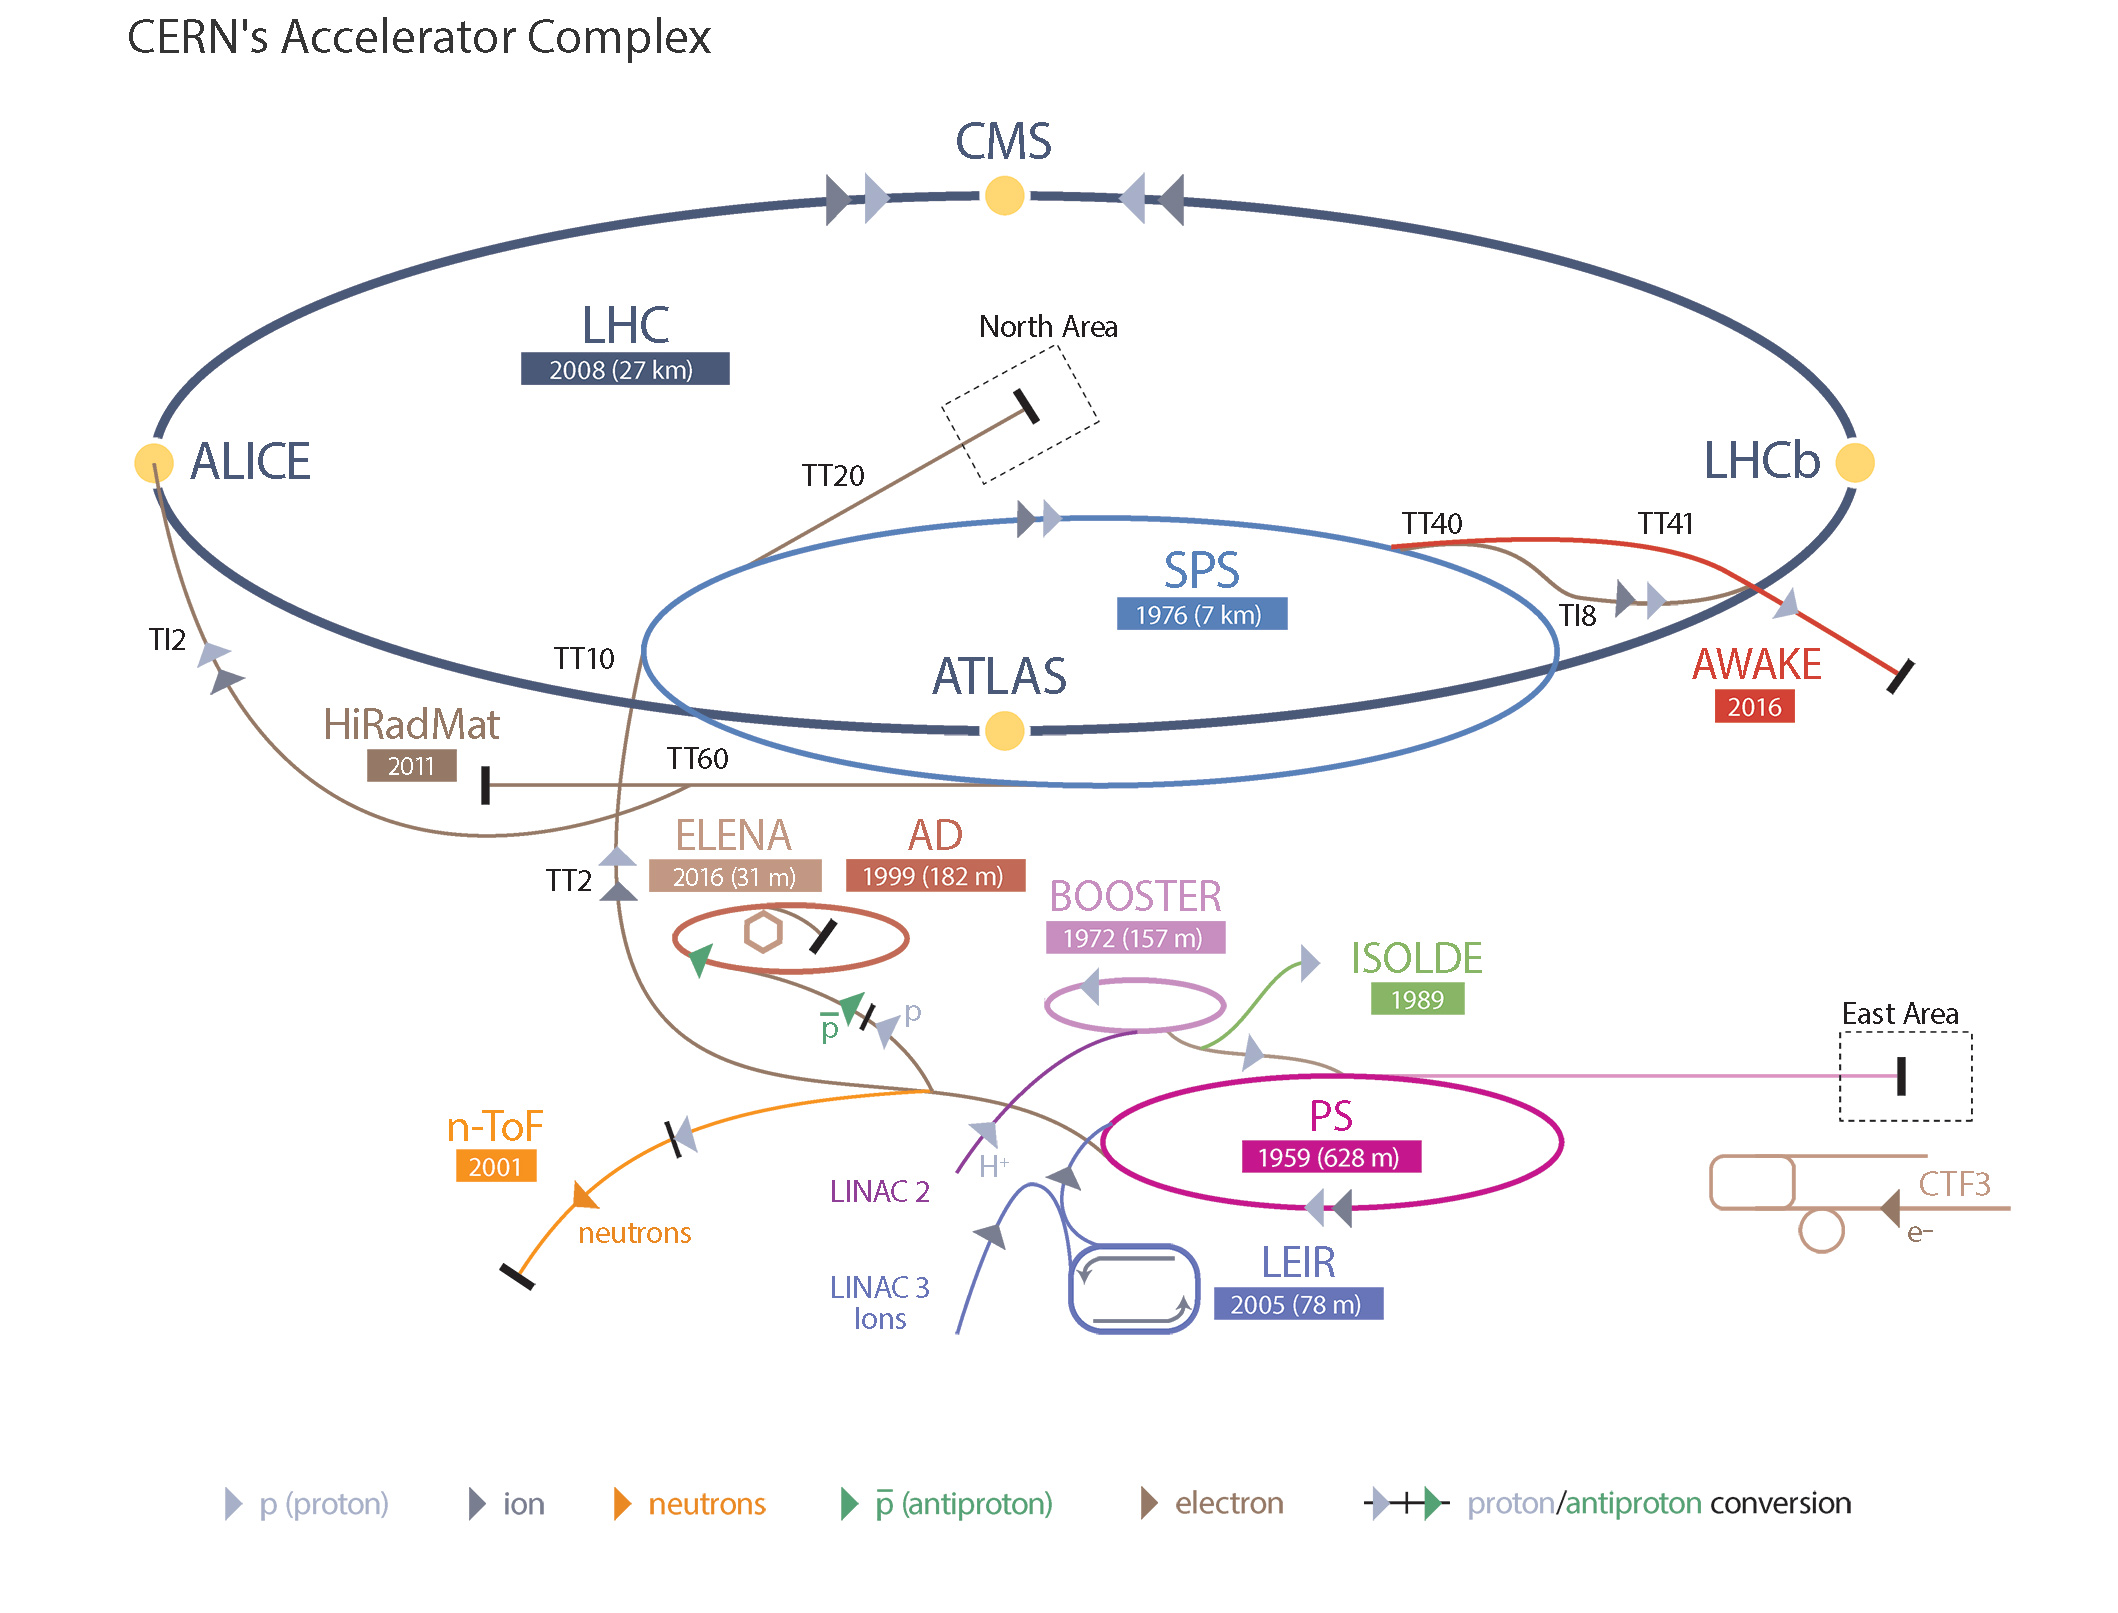
\includegraphics[width = 1.\textwidth]{figures/cms/LHC_accelarator_complex.jpg}
  \caption{The CERN accelerators complex. Protons are first extracted from a hydrogen tank and and accellarated up to 50 MeV by
    a linear accelarator (Linac 2), the Proton syncroton booser (BOOSTER) and Proton syncroton (PS) push the energy up to
    1.4 GeV and 25 GeV respectively. Protons are then transfered to the Super proton syncroton (SPS) where they are accelerated to
    450 GeV and injected into the LHC. Others machines are present at CERN complex to provide dedicated beams to various experiments.
    Furthermore both from the PS and the SPS the proton or ion beam is sent to a fixed target to provide secondary beams of pions, muons and electrons to several areas dedicated to fixed target experiments or R\&D projects. 
  }
  \label{fig:lhc_chain}  
\end{figure}

To reach the nominal luminosity, up to 2808 bunches per beam, with about $1.1\times 10^{10}$
protons each, are collided every 25 ns.
On the LHC ring four main experiments are located: ATLAS~\cite{atlas}, CMS~\cite{cms}, LHCb~\cite{lhcb} and
ALICE~\cite{alice}. CMS and ATLAS are general purpose experiments, with complementary features
and detector choices. CMS is described in detail in the next sections. The LHCb collaboration
aim to perform precision measurements on CP violation and rare decays, in order to reveal
possible indications for new physics phenomena. ALICE is dedicated to heavy ions physics and the
goal of the experiment is the investigation of the behaviour of the strongly interacting hadronic
matter resulting from high energy lead nuclei collisions. In those extreme energy densities the
formation of a new phase of matter, the quark-gluon plasma, is expected.

The LHC cycle consists of several phases: the machine is filled with protons while the energy is kept at
450 GeV, once the machine is full the beams are accelerated, squeezed and set on colliding orbits.
The instantaneous luminosity is maximized in ATLAS and CMS while in ALICE and LHCb it is kept
at lower values. Each cycle is called a ``fill''.

\section{The CMS experiment}

The CMS experiment is a general purpose detector for particle physics. The detector
includes several subsystems symmetrically centered around
the fifth interaction point of LHC. The detector is 22 m long and 15 m wide and is depicted in Figure~\ref{fig:CMS}.
It consists of a central, ``barrel'', part and two forward regions, the ``endcaps'', which
detect particles at small deflection angles.
The main detector component is the is the
superconducting solenoid that generate a magnetic field of 3.8 T. The tracking and calorimeter
systems are contained within the solenoid. This design benefits
the particle reconstruction as it minimizes the probability for a charged particle to
generate a shower before reaching the calorimeters while traversing the dense material of
the solenoid. Most of the detector is supported by
a steel skeleton which serves also as the return yoke for the magnetic field of 1.8 T
present outside the solenoid volume.
The muon detection system is placed outide the solenoid and inside the return yoke. The CMS detector has a weight
of about 12500 tonnes, mainly due to the steel skeleton and the solenoid.

\begin{figure}[!h]
  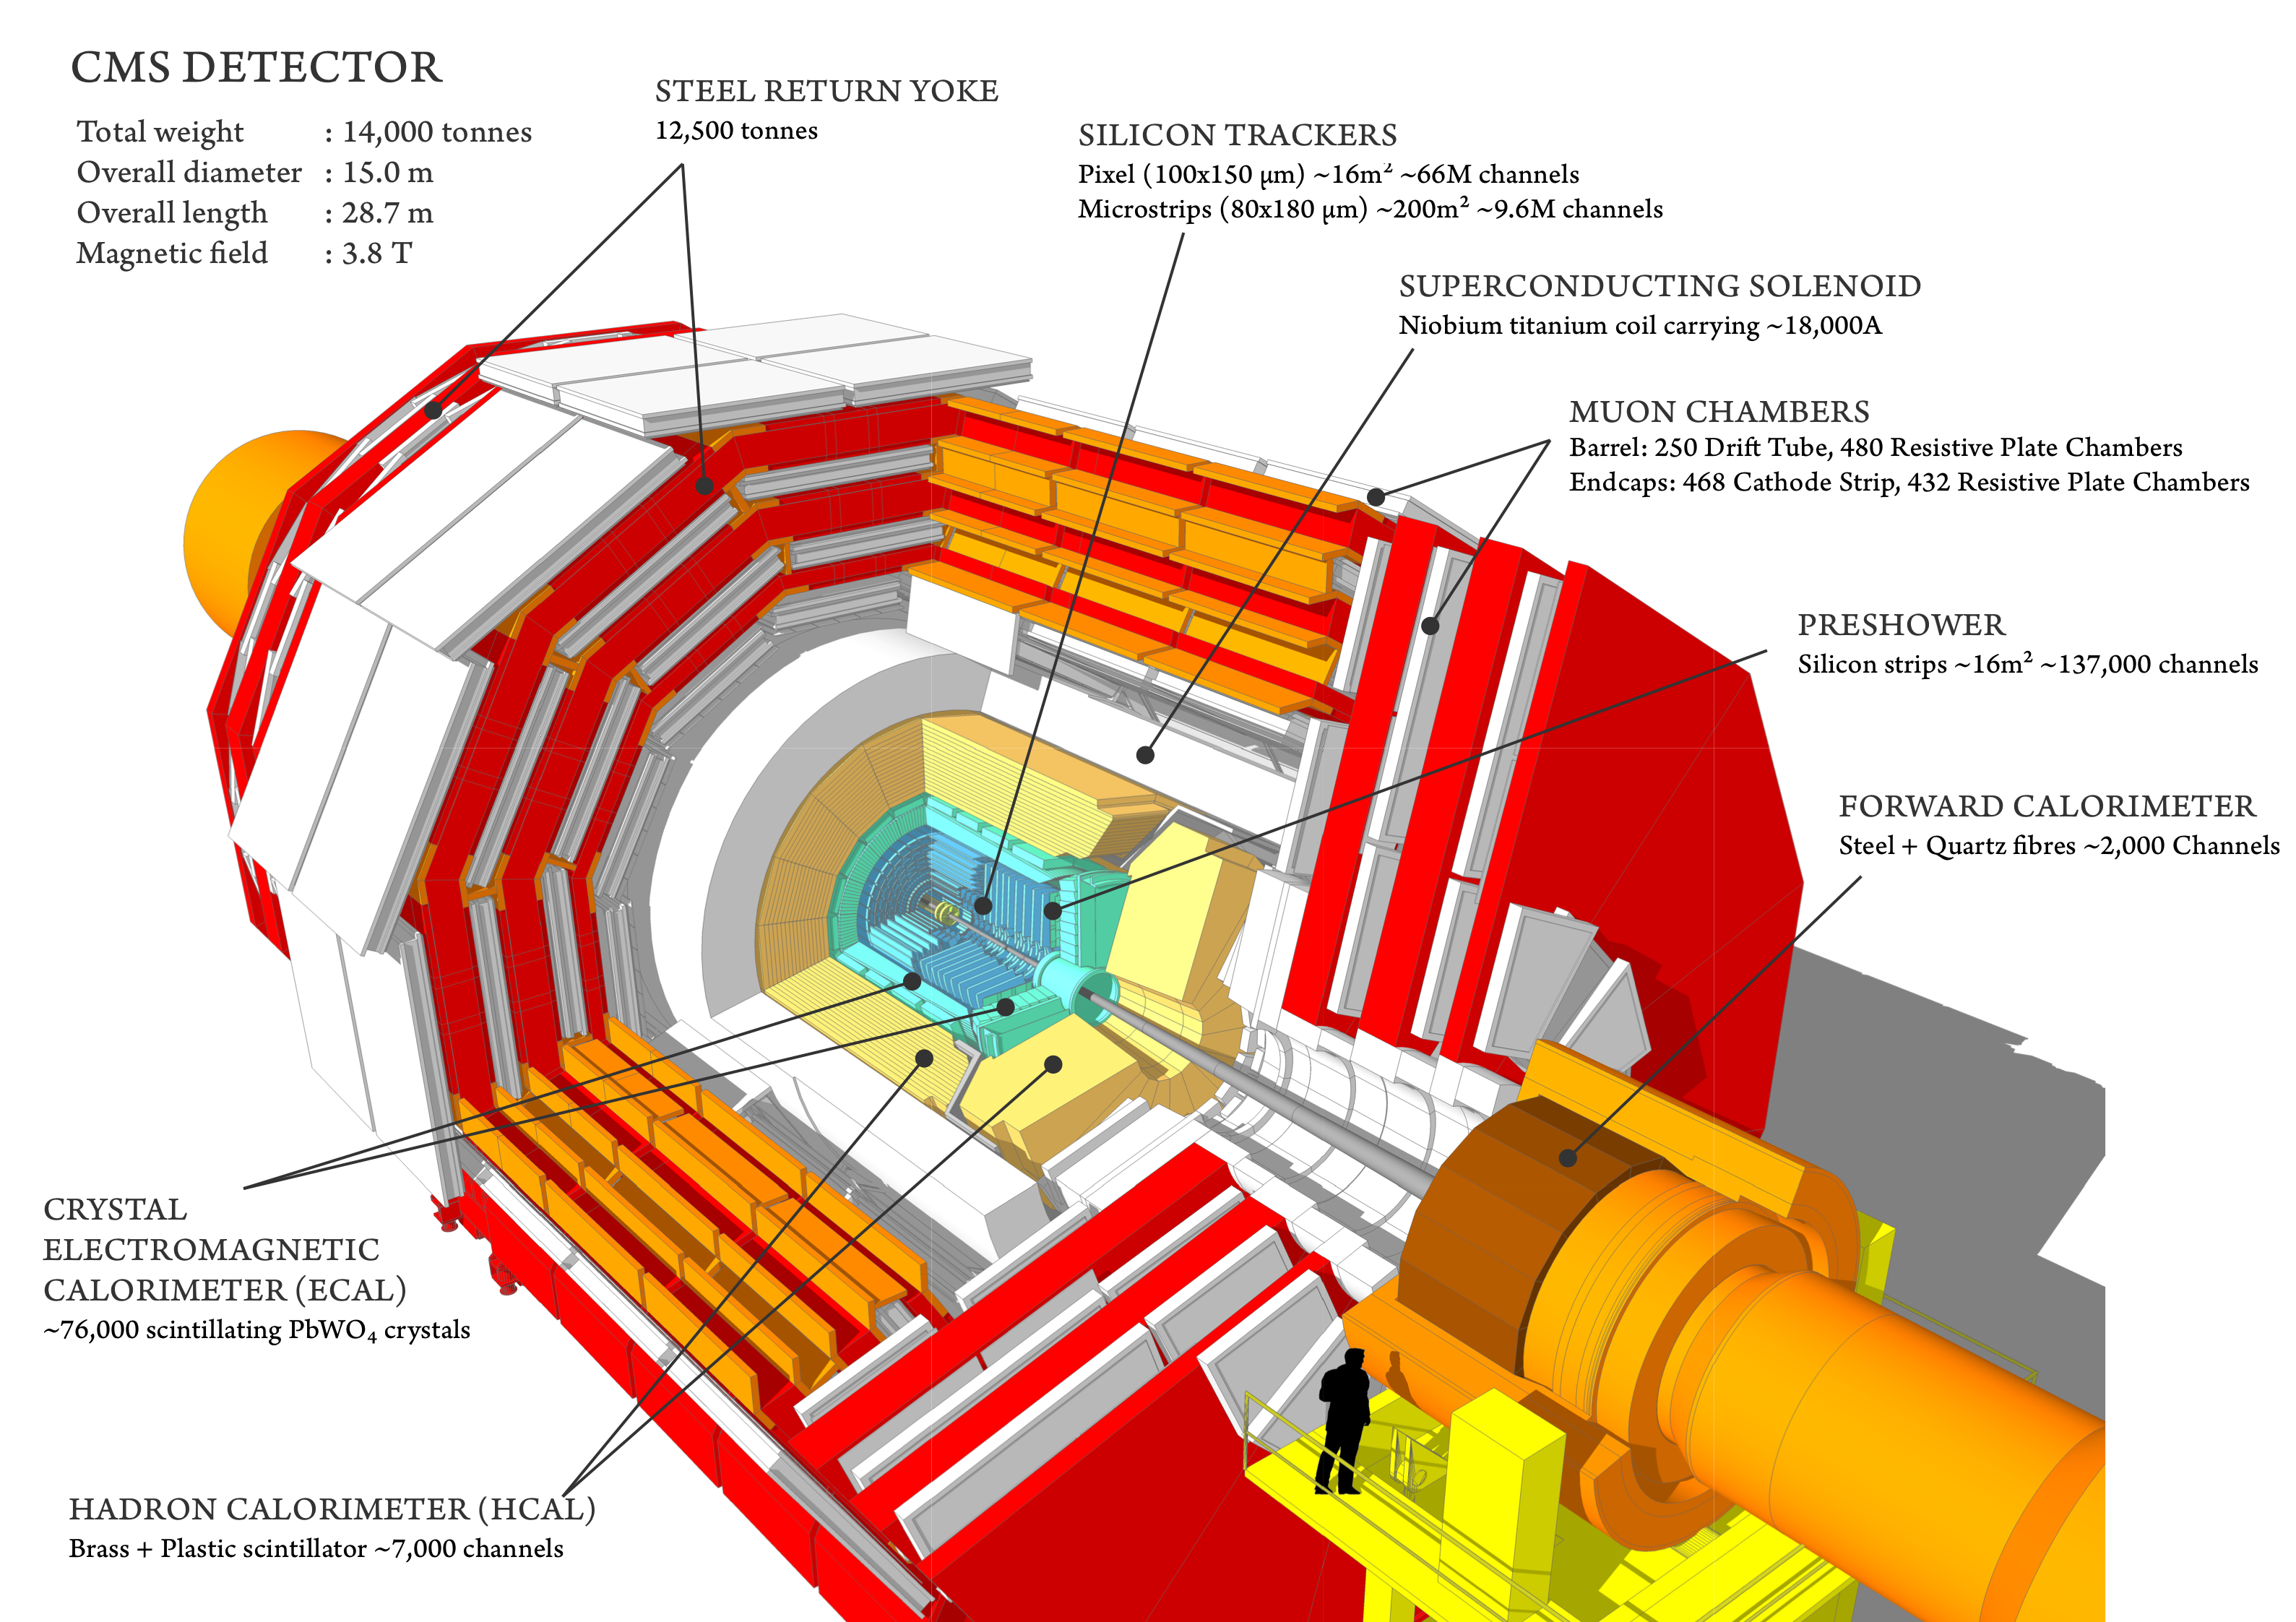
\includegraphics[width = 1.\textwidth]{figures/cms/cms_layout.png}
  \caption{Sketch of the Compact Muon Solenoid experiment \cite{cms_sketch}.}
  \label{fig:CMS}  
\end{figure}


The origin of the right-handed coordinate system of CMS is the central collision point,
with the z-axis oriented in the anticlockwise-beam direction. The x-axis is oriented
towards the center of the LHC accelerator ring, the y-axis points upwards.

The azimuthal angle ($\phi$) lies in the x-y plane and is measured
from the x-axis. A slice of the CMS detector in this x-y plane is shown in Figure~\ref{fig:CMS_xycut}.
The polar angle ($\theta$) is directed upwards from the z-axis. With the polar angle, the
pseudorapidity ($\eta$) can be defined:

\[
\eta = -ln( tan( \frac{\theta}{2} ) )
\]

The paricle mass $m$, momentum in the transverse plane $p_T$ and its $\eta$ and $\phi$ rappresent a convinient set of
variables to describe the particles produced in hadronic $p-p$ collisions where the fraction
of momentum carried by each of the colliding parton is in principle unknown.

\begin{figure}[!h]
  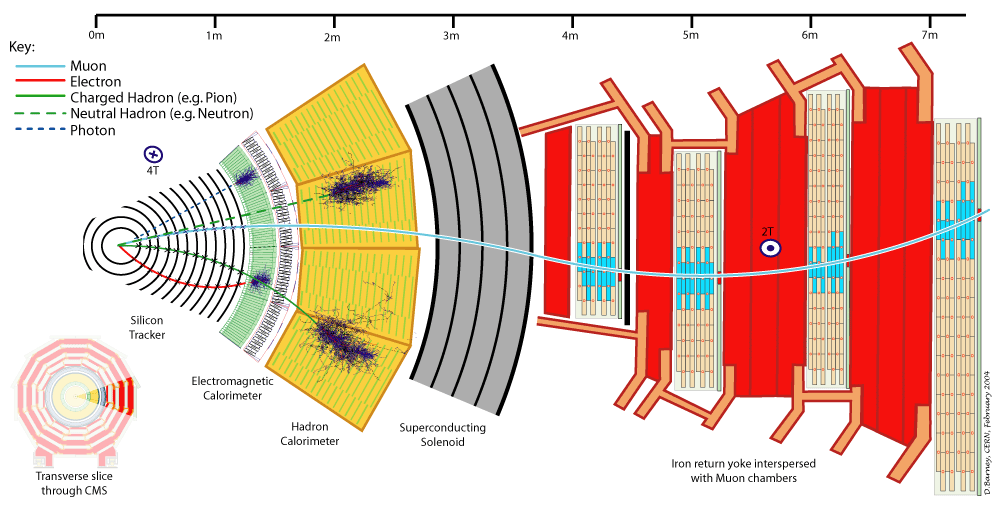
\includegraphics[width = 1.\textwidth]{figures/cms/CMS_Slice.png}
  \caption{A slice of the CMS detector in the x-y plane. Various particle type detection are depicted, the
    details of each system are given in the text.}
  \label{fig:CMS_xycut}  
\end{figure}

\subsection{The tracking system}
The tracking detector surrounds the beampipe, the innermost layer is installed
about 4 cm from the interaction point (IP). It has a length of 5.8 m, a diameter of 2.6 m,
and covers a range of $|\eta| < 2.5$ with an area of over $200~\mathrm{m}^{2}$ active silicon sensors, its
layout is shown in Figure~\ref{fig:cms_tracker_layout}. It is
designed to measure the trajectories of particles as highlighted in Figure~\ref{fig:CMS_xycut}. As such,
it has to provide a high spatial resolution and a fast signal readout while withstanding a fluence
of about $10^6$ particles/( cm$^2$ s) (at a distance of 8 cm from
the IP).
The core of the tracking system, the silicon pixel detector, is made of 66 million pixels
with a size of $100 \times 150 \mu$m$^2$ , enabling the reconstruction of primary and secondary
vertices with a precision that ranges between 100 $\mu$m to 1 mm in the z direction and of few tens of $\mu$m
in the x and y directions. The silicon pixel detector is followed by a silicon strip detector with coarser
granularity. The track recognition is performed by about 15200 highly sensitive
modules containing 10 million detector strips. The tracking detector has a radiation length ($X_0$) of 0.4 at $\eta = 0$,
which increases at larger $\eta$ to approximately 1.8 $X_0$ at $|\eta|$ = 1.4 as visible from Figure~\ref{fig:cms_tracker_material}.

\begin{figure}[h]
  \centering
  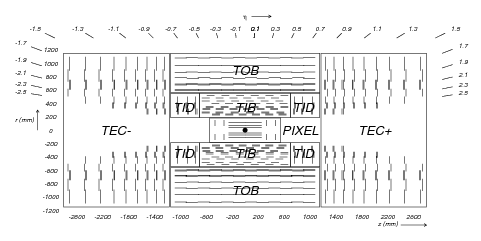
\includegraphics[width = 1.\textwidth]{figures/cms/trackerLayout.png}
  \caption{Schematic cross section through the CMS tracker in the r-z plane. Each line-element represents a detector module.
    Closely spaced double line-elements indicate back-to-back silicon strip modules,
    in which one module is rotated through a ``stereo'' angle, so as to permit reconstruction of the hit positions in
    three dimensions. Within a given layer, each module is shifted slightly in r or z with respect to its neighbouring modules,
    which allows them to overlap, thereby avoiding gaps in the acceptance \cite{cms_trk}.}
  \label{fig:cms_tracker_layout}
\end{figure}

\begin{figure}[h!]
  \centering
  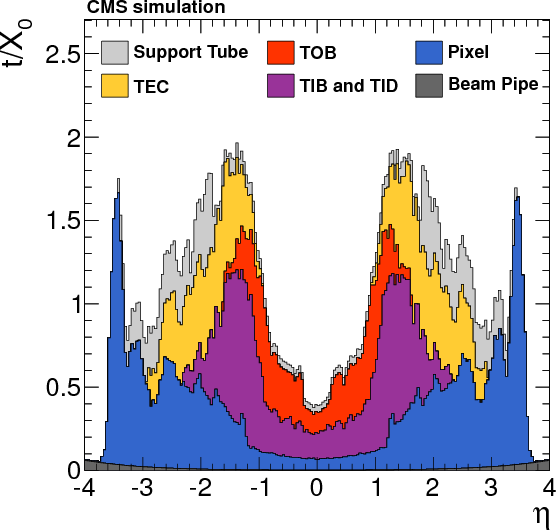
\includegraphics[width = .7\textwidth]{figures/cms/MaterialBudget.png}
  \caption{Total thickness $t$ of the tracker material traversed by a particle produced at the nominal interaction point,
    as a function of pseudorapidity $\eta$, expressed in units of radiation length $X_0$.
    The contribution to the total material budget of each of the subsystems that comprise the CMS tracker is shown,
    together with contributions from the beam pipe and from the support tube that surrounds the tracker~\cite{cms_trk}.
    The configuration shown in the picture reflects that of the CMS tracker prior the upgrade of the
    pixel detector in 2017, that significantly reduces the material budget in forward region.}
  \label{fig:cms_tracker_material}
\end{figure}

\subsection{The calorimeter system}
\label{sec:cms_calo}
The calorimeter system is devided in two section: the electromagnetic part ECAL which measures the energy
of electrons and photons and the hadronic part dedicated to the measurment of the energy of charged and
neutral hadrons. The two detectors differ both in porpouse and technology.

The ECAL is an homogeneous and hermetic calorimeter, made of scintillating lead tungstate
crystals. The chosen crystal is suitable for operation at LHC due to its fast emission
(80\% of the scintillation light is emitted within 25 ns) and its resilience to irradiation. Moreover,
thanks to crystal short radiation length ($X_0 = 0.89$ cm) and small Molière radius ($r_M = 21.9$
mm), most of an electron or photon energy can be collected within a small matrix of crystals.

As the other CMS sub-detectors the ECAL is devided in two main section:
\begin{itemize}%[label=\color{black}\textbullet]\itemsep5pt
\item Barrel (EB): it covers the region $|\eta| < 1.4442$ with 61200 crystals arrenged in 170 rings of 360 crystals each.
\item Endcap (EE): it covers the region $1.556 < |\eta| < 3.0$ with 14648 crystals arrenged in 4 Dees of 3662 crystals each.
\end{itemize}

All the crystals are mounted with a tilt of $3^{\circ}$, both $\eta$ and $\phi$ projections, in
a quasi-projective geometry to avoid gaps aligned with the particles trajectories. The EB
is located at $R = 1.3$ m from the IP while the endcaps are installed at $z = \pm 3.10$ m Figure~\ref{fig:cms_ecal_layout}.

\begin{figure}
  \centering
  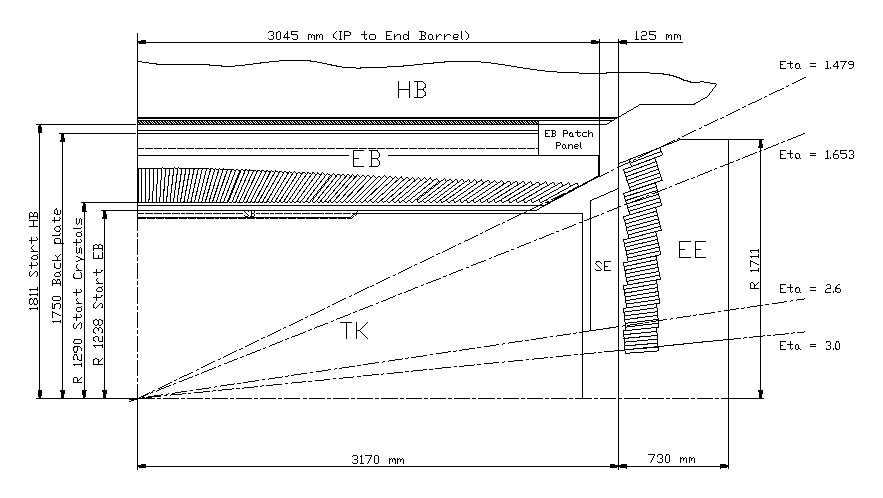
\includegraphics[width = 1.\textwidth]{figures/cms/ecal_layout.eps}
  \caption{Schematic view in the r-z plane of the CMS electromagnetic calorimeter and pre-shower. Only one fourth of the
    entire system is shown. Only the \PbWO crystals are drawn, without the supporting frame, cooling and readout
    electronic boards \cite{cms_ecal}.}
  \label{fig:cms_ecal_layout}
\end{figure}    

The relatively low light yield of $\sim 30 \gamma/$MeV makes the use of intrinsic high-gain
photodetector necessary, capable of operating in an high magnetic field. Avalanche PhotoDiodes (APDs) are
used to collect light in barrel crystals while Vacuum PhotoTriodes (VPTs) are used in the endcaps.
Two APDs are glued on the crystals rear face and their signals are summed before reaching the front-end electronics.
In the endcaps only one VPT is used for each crystal.

APDs have a gain of 50 at nominal operation bias voltage, while the relative gain variation due to changes in the bias voltage
is of $\Delta G/\Delta V = 3.1\% /V$. The APDs gain also depends on temperatures as
$\Delta G/\Delta T = -2.4\% /C^{\circ}$. 

VPTs are more radiation resilient and thus were chosen as photodector in the endcap regions
but have a gain variation of about $25\%$ across the endcaps.

ECAL operates with a temperature of $18 C^{\circ}$ which is maintained by a dedicated cooling system.
The temperature dependence of the crystal light yield ($−2\% C^{\circ}$) and of the APD gain
demand a precise temperature stabilization to the level of $0.05 C^{\circ}$ in the EB. In the
endcaps, the dependence of the VPT response on the temperature is negligible,
so a stabilization at the level of $0.1 C^{\circ}$ is sufficient. These specifications limit the contribution
of temperature variation to the constant term of the energy resolution to be less than 0.2$\%$.

The ECAL system is complemented by a pre-shower (ES) placed in front of each of the ECAL endcaps.
The ES is made two layers of silicon strips alternated with passive layers of lead radiators ($2 X_0$ and $1 X_0$)
that extend from $\eta$ 1.6 to 2.8.
The ES is used to discriminate between collimated photons caming from decays of neutral hadrons and
real photons.


The HCAL measures the energy of hadrons by stopping them within its
hermetic volume and reading out the deposited energy. Its dimensions (Figure~\ref{fig:cms_hcal_layout})
are constrained by the ECAL ($R = 1.77$ m) and the surrounding magnet coil
($R = 2.95$ m). The chosen design is the one of a sampling calorimeter with brass absorbers
and scintillating tiles for the energy measurement. The readout is performed via
optical fibers by hybrid photodiodes.

\begin{figure}
  \centering
  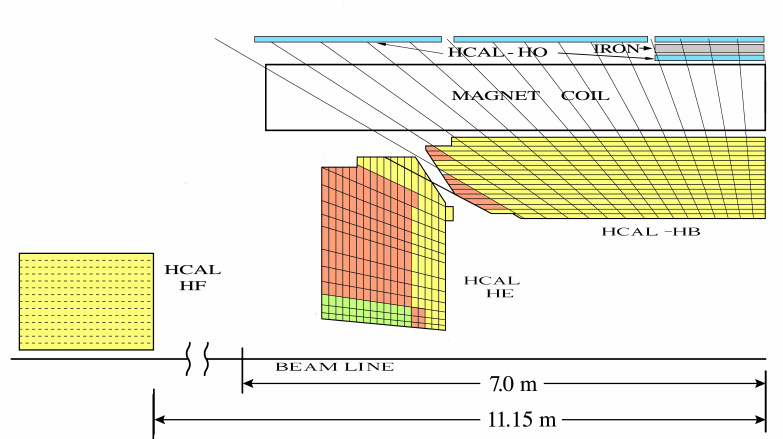
\includegraphics[width = 1.\textwidth]{figures/cms/hcal_layout.png}
  \caption{Schematic view in the r-z plane of the CMS hadronic calorimeter. Only one fourth of the
    entire system is shown. All four partitions are visible: the barrel and endcaps part (HB and HE), the
    tail catcher installed outside the CMS solenoid and the forward calorimeter.}
  \label{fig:cms_hcal_layout}
\end{figure}    

The HCAL effective thickness increases with polar angle as $1/cos\theta$ in the barrel, 
it varies from 5.82 interaction length at $\eta = 0$ to 10.6 at $\eta = 1.3$ while it is
costant at about 10 interaction length in the endcap regions.
An additional  small hadron
calorimeter is placed behind the solenoid to capture very high energetic hadrons showers not
contained with the inner calorimeters and the magnetic coil, this additional piece of the HCAL
is used to reduce the mis-identification of hadronic jets as muons. The
granularity in the barrel region ($|\eta|<1.3$) is $\Delta\eta × \Delta\phi = 0.087 \times 0.087$, while
in the endcap regions ($1.3<|\eta|<3.0$) it is
$\Delta\eta × \Delta\phi = 0.17 \times 0.17$. The forward region ($3.0 < \eta < 5.2$)
is covered by a Cherenkov-based calorimeter (HF), the absorber is made of steel while the
active medium are quartz fibers.
This forward calorimeter is placed at a distance in z of 11.2 m from the IP it has been design
to withstand 10 MGy of absorbed dose and is expected to last for ten years during the LHC operation.

\subsection{The muon system}
The CMS muon system~\cite{muon_tp} provides full geometric coverage for muon measurement up to $|\eta| = 2.4$.
The detectors are embedded in the magnet return yoke, so that muon momentum and charge
measurements can also exploit the strong magnetic return field (Figure~\ref{fig:cms_muon_layout}).
This is particularly important
for muons with transverse momentum in the $\sim 1$~TeV range, for which the complementary tracker
measurements degrade.

\begin{figure}
  \centering
  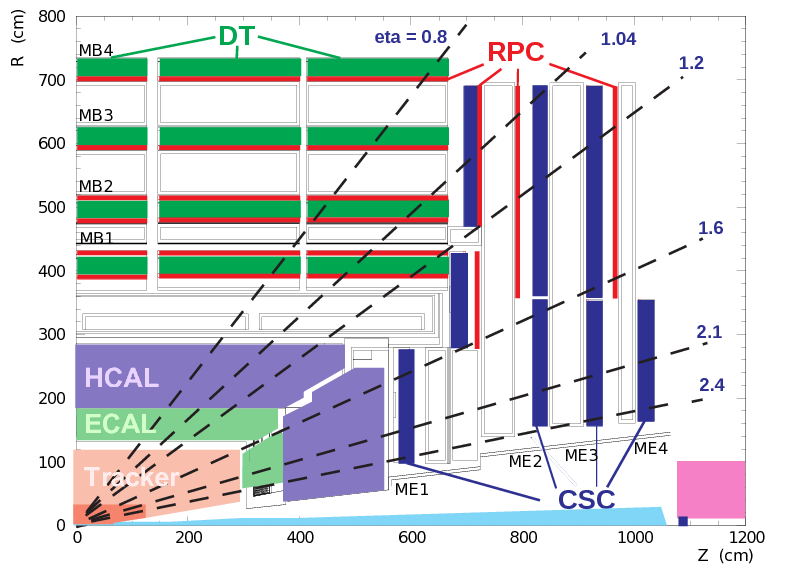
\includegraphics[width = .45\textwidth]{figures/cms/muon_layout.png}
  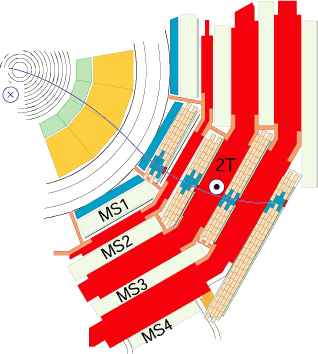
\includegraphics[width = .45\textwidth]{figures/cms/muons_xyview.png}
  \caption{Layout of one quadrant of CMS in the longitudinal (left) and transverse (right) planes.
    The four DT stations in the barrel (MB1-MB4, green),
    the four CSC stations in the endcap (ME1-ME4, blue), and the RPC stations (red) are shown.}
  \label{fig:cms_muon_layout}
\end{figure}

The CMS muon spectrometer exploit three different detector tecnologies; the need of a fast response for
generate a muon trigger and that of high spatial resolution for excellent momentum determination could not
be satisfied by a unique technology.
Both in the barrel ($|\eta| < 1.2$) and endcaps $0.9 < |\eta| < 2.4$ resistive-plate-chambers (RPC) are used
to signal the presence of high energy muons at trigger level (up to $|\eta| < 2.1$).
Drift-tube (DT) and chatode-strip-chambers (CSC) based detectors
provide the mmomentum measurement in the barrel and endcaps respectively. The angular resolution
in $\phi $ is of about 1 mrad.

The RPC and DT detectors are alternated in concentric rings at a radius between 4 and 7 m from the IP
in the barrel region. The rings are arranged in a way that avoids geometrical gaps in the $\phi $ projection, gaps
in the $\eta $ one are avoided by placing the detectors parallel to the z-axis.
In the endcaps the CSC are alternated to the RPC detectors in six consecutive disc on each side of the IP, the CSC
detectors inner region is placed at a radius of 1 m from the beamline.

\subsection{The trigger system}
The collision rate (40~MHz) is higher that the rate at which event can be recorded and stored for
offline processing (1~kHz). A two stage trigger system has been implemented to select events containing
a possible hard scattering within the tens of concurrent collisions happening at each bunch-crossing.

The first level (Level-1 trigger) is hardware  implemented in the readout electronics of each sub-system except for
the tracker. The hardware used is based custom chips programmed with a dedicated firmware.
The Level-1 triggers involve the calorimetry and muon systems, as well as some correlation
of information between these systems. The Level-1 decision is based on the presence of trigger
primitive objects such as photons, electrons, muons, and jets above adjustable transverse energy thresholds.
It also employs global sum of $E_T = \sqrt{m^2 + p_T^2}$ and $E_T^{miss}$~\cite{trigger}. Reduced-granularity and
reduced-resolution data are used to reconstruct trigger candidates.
The Level-1 trigger reduces the event rate to 100~kHz.

The second level (high level trigger or HLT) reduces the rate to the 1 kHz and performs a simplified and faster
version of the final event reconstruction. The main idea is run the event reconstruction on demand in cascade for
different types of objects such that non-interesting events can be discarded without running the whole
event reconstruction. The HLT runs on commercial CPUs, 
a set of different trigger algorithm are implemented such that the events are classified accordinlgy
to their topology (i.e. events with a muon pair, electron pair, large $E_T^{miss}$, ...).

In addition to triggers where all events that satisfies the requirements are saved (unprescaled
triggers), a set of utility triggers, whose rate would be too high due to band saturation, have
been developed, where a good event is saved only once every N times (prescaled triggers, with
a prescale parameter N). These trigger paths are used for detector studies and to study kinematical
regions of object reconstruction, such as low $p_T$ leptons.

\subsection{The event reconstruction}
\label{sec:cms_pf}
Events selected by the HLT trigger are stored and analyzed on a world-wide network of computers.
Events can be reconstructed several times if a better calibration of the detector or reconstruction algorithm is
developed. The CMS event reconstruction core is the so called particle-flow algorithm~(PF)~\cite{PF}. The PF main idea
is to combine information coming from the different systems, for instance charged hadrons are detected both
in the tracker as tracks and by the HCAL as energy deposit. Combining the momentum measurement of the tracker
with the energy measurement of the HCAL improves the overall energy resolution on hadronic jets.
Electrons and photons are primarly reconstructed as energy clusters in the ECAL, the tracker information is
used to discriminate electrons from photons. A clustering algorithm is used to recover energy loss by bremsstrahlung
or photon conversion.
Jets of charged and neutral hadrons are clusterd using various algorithm accordingly to the particular needs of an analysis.
Leptons and photons are distinguished from jets by requiring isolation criteria.
Finally the missing transverse energy is calculated as:
\[
  -\Sigma \vec{E_T^{miss}}
\]

where the sum runs over all the objects reconstructed by combining all the system information using the PF algorithm.

\clearpage\providecommand{\sumEt}{\ensuremath{\sum E_T}\xspace}
\providecommand{\sumEtring}{\ensuremath{\sum_{\eta-ring} E_T}\xspace}
\providecommand{\sumEtEB}{\ensuremath{\sum_{EB} E_T}\xspace}

\chapter{ECAL energy reconstruction and calibration}

In this chapter the reconstruction and calibration of the energy measured by the ECAL
is presented. Photons are detected only by the ECAL and the analysis sensitivity strongly depends
on the ECAL energy resolution, furthermore some of the variables used to discriminate photons
from jets (see Section~\ref{sec:dipho_selection}) also relies on ECAL information and the stability
over the whole data-taking of such variables is important to ensure an optimal selection efficiency.

\section{Energy reconstruction}
\label{sec:ecal_reco}
A photon or electron entering the ECAL produces a shower in the \PbWO crystals. The energy of
these electromagnetic showers is deposited in crystal matrices. On average the electrons/photons
leave $94\%$ of their total energy in a $3\times3 $ crystal matrix and $97\%$ of their total energy in a $5\times 5$
crystal matrix surrounding the crystal hit by the particle.
Electrons are reconstructed combining ECAL and tracker measurements [59],
while the photon reconstruction relies only on the ECAL [60].

Since the electromagnetic shower generated by a photon or electron span more than one crystal the
energy reconstruction involves both the measurement of the scintillation light in the crystals as well
the clustering of signals originated by the same particle. The clustering takes into account
also bremsstrahlung and photon conversion processes that take place in the tracker and which, due to the
intense magnetic field, spread the energy deposition along $\phi$.
The clustering algorithm [127,128] begin first with the formation of
``basic clusters'', corresponding to local maxima of energy deposits. The basic clusters are then
merged together to form a ``supercluster'' [113], which is extended in $\phi$, to recover the radiated energy.
The different geometric arrangement of the crystals in the barrel and
endcap regions implies that a different clustering algorithm is used for two regions. The algorithms do not
make any hypothesis as to whether the particle originating from the interaction point is a photon
or an electron, consequently electrons from \Zee events can provide excellent measurements
of the photon reconstruction and identification efficiencies, and of the photon energy scale and
resolution. The clustering algorithms achieve a rather complete ($\sim 95\%$) collection of the energy
of photons and electrons, even those that undergo conversion and bremsstrahlung in the material
in front of the ECAL.
The energy in a supercluster can be expressed as:

\begin{equation}
  E_{e,\gamma} = F_{e,\gamma} \cdot \left[ G \cdot \sum_{i} ( S_i(t)\cdot C_i \cdot A_i ) + E_{ES} \right]
\end{equation}
\label{eq:sc_energy}

the sum runs over the crystals composing the supercluster and the terms represent:

\begin{itemize}
\item $A_i$: the signal amplitude in ADC count estimated with the method explained in Section~\ref{sec:signal_reco}.
\item $C_i$: the intercalibration coefficient which equalizes relative differences in the crystals response.
\item $S_i(t)$: the time dependent correction for the loss of transparency explained in Section~\ref{sec:laser}.
\item $G$: the scale coefficient to convert the digital scale measured in ADC count to energy scale expressed in GeV.
  It has two values:
  one for the EB and one for the EE set comparing the scale between data and simulation in \Zee events.
\item $E_{ES}$: Only for electrons or photons in the acceptance region of the ECAL preshower the energy measured
  by the ES is summed to that of the ECAL supercluster.
\item $F_{e,\gamma}$: supercluster energy correction. Several effect like shower non-containment, pile-up and
  loss of energy in the tracker are corrected with a regression technique trained on simulation. The factor also
  takes into account the slightly different shower development of electron and photons.
\end{itemize}

\subsection{Signal reconstruction}
\label{sec:signal_reco}
The scintillation light, emitted by \PbWO , is measured by the photo-detectors as explained in
Section~\ref{sec:cms_calo} and read
out as an analog signal by the front-end electronics. The signal is pre-amplified, shaped
and processed by a multi-gain amplifier. A dynamic range spanning from
approximately 50 MeV to 3 TeV [111] is achieved thanks to three
amplifiers that process the signal in parallel: the amplifiers gains are 1, 6 and 12.
For very high energy photons, the ECAL readout electronic system saturates.
The dynamic range limit is reached when the energy
deposit in a single crystal has a value of about 1.7(2.8) TeV in the barrel (endcaps) and for
non irradiated crystals. The highest, non-saturated signal among the three amplifiers is then digitized by a 12-bit
ADC operating at 40 MHz, ten consecutive samples are read out by the front-end electronics.
% If one of the ten samples is read out from one of the lower gain amplifiers all the following
% samples read with the same gain unless a even lower one is required.


\begin{figure}[!h]
  \centering
  \includegraphics[width = 0.45\textwidth]{figures/ecal/multifit_EB.pdf}
  \includegraphics[width = 0.45\textwidth]{figures/ecal/multifit_EE.pdf}
  \caption{Example of fitted pulses for simulated events with 20 average pileup interactions and 25 ns bunch spacing, for a signal in the barrel. Dots represent the 10 digitized samples, the red distributions (other light colors) represent the fitted in-time (out-of time) pulses with positive amplitude. The dark blue histograms represent the sum of all the fitted contributions \cite{Multifit}.}
  \label{fig:multifit_for_dummies}
\end{figure}

The signal amplitude is reconstructed from the set of ten samples measured for each channel at each event.
The method developed for collisions at 13 TeV and LHC bunch spacing of 25 ns estimates
the in-time signal amplitude and up to nine out-of-time
amplitudes for each signal pulse by a $\chi^2$-minimization via the non-negative-least-squares
technique to the ten digitized samples~\cite{Multifit}, the signal shape used to estimate the contribution of each
energy deposit to each sample is assumed to be the same regardless of when the energy is deposited with respect
the in-time one.
The goal of such approach is to suppress the contributions from OOT energy deposits
to the measurement of the interesting signals.
The out-of-time (OOT) amplitudes corresponds to
energy deposits coming from five bunch crossings that precede the in-time one and four that follow it.
Two examples of a fitted pulse shape for
a simulated event are shown in Figure~\ref{fig:multifit_for_dummies} for the EB and the EE category, respectively.
This method is not used when at least one of the samples is read-out through either the gain 6 or gain 1
amplifiers since a known non-linearity of electronics (slew-rate) introduces a distortion in the signal shape
and therefore bias the estimation of the in-time and out-of-time amplitudes.
In such cases since the in-time signal is usually much larger than the out-of-time ones,
the amplitude of the sixth sample is taken as measurement of the in-time energy deposit.

\section{The laser monitoring system}
\label{sec:laser}
The optical transmission within crystals at the scintillation wavelengths is affected by the production
of color centers under ionizing electromagnetic radiation. This transparency loss process is not permanent,
in fact spontaneous annealing of the colour centers occurs also at room temperature and leads
to a transmission recovery, which is evident when the crystals are not irradiated, such as during
machine-fill gaps or winter stops.
Permanet demage can be induced by hadrons traversing the crystals, its impact on the ECAL energy resolution
is expected to be below the design limits up to 500\fbinv.

Crystals produced for ECAL are optimized to reduce the relative variations in light transmission
during an LHC collision running period to less than $6\%$ for the barrel
crystals (dose rates of 0.15 Gy/h) and less than $20\%$ for the endcpas at $|\eta| = 2.5$ (dose rates of
1.9 Gy/h) [b62].

The laser light pulses are directed to individual crystals via a multi-level optical-fibre distribution
system. The basic operations for barrel geometry are the following: laser pulses transported via
an optical fibre are injected at a fixed position at the crystal’s front face, the injected light is
collected, with the pair of APDs glued to the crystal’s rear face, as for scintillation light from an
electromagnetic shower. Although the optical light path is different from that taken by shower
scintillation photons, this design guarantees that the light transmission is measured in the relevant region.
The underlying principle is similar for ECAL endcaps; however, laser light is injected
at a corner of each endcap crystal’s rear face, and the light is collected (as for scintillation) via
a VPT glued on the crystal’s rear face. The intensity of the injected laser is monitored through a set of PN diodes,
the ratio between the APDs amplitude and the one measured with
the PN diode is used to monitor the transparency variation. Each PN diode monitors a region composed by 100 to 200 crystals.

The energy correction factor extracted by means of the laser monitoring system depends on
the light collection mechanisms of both electromagnetic showers and injected laser.
It is possible to define from first principles a relation between
the APD signal amplitude of a electromagnetic shower ($S$) and the one for injected laser light ($R$) [62].
The demonstration begins considering the average light optical path ($\Lambda$) and the average light attenuation
coefficient ($\lambda$), which is directly related to the light transmission. If we consider a shower, with
initial amplitude $S_0$ , which goes through the crystal, the measured amplitude $S$ is:
\[
  S = S_0 e^{-\frac{\Lambda_S}{\lambda_S}}
\]

a similar relation holds for laser light, although the parameters differ since the optical paths for scintillation
light and laser light are different:
\[
  R = R_0 e^{-\frac{\Lambda_R}{\lambda_R}}
\]

on average the scintillation light production is isotropic and thus
the scintillation light travels a lorger path in the crystal before reaching the photodetector than the
injected laser light, the relation between the two can be written as:
\begin{equation}
  \frac{S}{S_0} = \left(\frac{R}{R_0}\right)^{\alpha}
\end{equation}
\label{eq:light_relation}

where $\alpha = \frac{\Lambda_S \lambda_R}{\Lambda_R \lambda_S}$ is an empiric parameter.

The laser light is injected regularly during the CMS dataking either during periods between LHC fills or
during the abort gap (a series of several empty bunch crossings during which the special magnets 
are turned on to dump the beam), the response is monitored with a granularity of about 40 minutes.
Three laser wavelength are available: blue (447 nm), green (527nm) and infrared. The blue laser is
preferred since it is the closest one to the scintillation spectrum.

Folowing Equation~\ref{eq:light_relation}, the correction for the transparency loss is computed as:
\[
  LC(t) = \left(\frac{R(t)}{R(t_0)}\right)^{\alpha}
\]

The reference response $R(t_0)$  is currently set to the one measured at the beginning of 2011 and its history is
reported in Figure~\ref{fig:laser}.
The response $R(t)$ is computed as the ratio between the APDs signal and the PN signal ($APD(t)/PN(t)$), as describet above
a PN diode is used to monitor the intesity of the injected light to avoide response variation due to laser instabilities.
Since the absolute intensity of the laser light injected in each crystal is unknown and may vary from channel to channel
(different fibers length, imperfect mechanical and optical matching, ...) it is impossible to estimate the value of $\alpha$
with a single measurement. Furthermore the value of $\alpha$ depends on the absolute transparency of the crystal, which
varies under irradiation.
The average value of $\alpha$ both for barrel and endcaps crystals was determined thanks to a series of measurment perform
at beam test before the CMS installation and in-situ during the first years of datataking. The limited set of data available
allowed only to determine the average value for the EB and the EE (1.52 and 1.16 respectively).
The majority of the ECAL crystals were produced in
Russia by BCTP while a minor fraction was produced in China by SIC, for these last crystals the value of $\alpha$ was
measured to be 1. From the same studies the spread of the value of $\alpha$ among crystals of the same producer
is known to be around $10\%$. 
An in-situ measurement of $\alpha$ for each single crystal, obtained with data collected during 2016, is reported in Section ???.

\begin{figure}
  \centering
  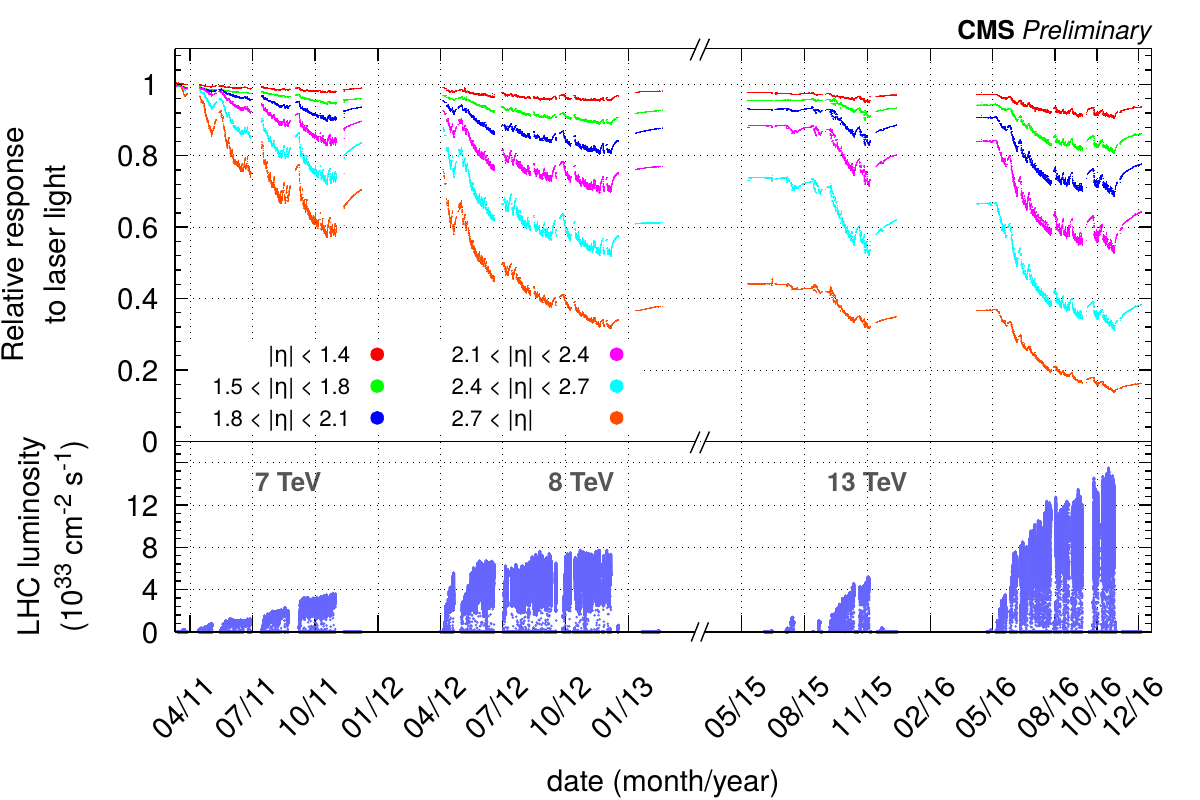
\includegraphics[width = .9\textwidth]{figures/ecal/histories_2011-2012-2015-2016_161212.png}
  \caption{Relative response to laser light (440 nm in 2011 and 447 nm from
    2012 onwards) injected in the ECAL crystals, measured by the ECAL
    laser monitoring system, averaged over all crystals in bins of
    pseudorapidity, for the 2011, 2012, 2015 and 2016 data taking periods,
    with magnetic field at 3.8 T. The response change observed in the
    ECAL channels is up to $10\%$ in the barrel and it reaches up to $50\%$ at $\eta\sim 2.5$,
    the limit of the tracker acceptance. The response change is up to $90\%$ in the region closest to the beam pipe
    \cite{laser_and_phisym}.}
  \label{fig:laser}
\end{figure}

\section{ECAL single channel intercalibration and response monitoring}
\label{sec:minchia_la_calibrazione}

The laser monitoring system provide a way to equilize the response over time but does not allow to
correct for absolute response differences among the ECAL channels. The crystal-by-crystal response variation
for crystals at the same $\eta$ ($\eta-ring$) are minimized by means of three techniques, all exploiting collision data:

\begin{itemize}
\item $\Phi$-symmetry: this method is based on the assumption that for a large sample of soft interaction
events (zero-bias) the total deposited transverse energy (\sumEt) is the same for all the crystals in a
$\eta$-ring, any observed asymmetry is attributed to a difference in the response of the crystals.
Intercalibration in $\phi$ is performed by comparing the \sumEt deposited in one crystal
with the total transverse energy collected by crystals at the same value of $\eta$ (\sumEtring).

\item Intercalibration with $\pi_0 and \eta$ mesons:
  In order to take advantage of the high rate of $\pi_0$ decays, a specialized HLT trigger stream has
been developed. In addition, a separate calibration stream has been implemented to select also
$\eta\to\gamma\gamma$ decays. An iterative procedure is used to determine the intercalibration constants.
The $\pi_0$/$\eta$ invariant mass distribution is fitted with a Gaussian function, for the signal, and a
fourth-order polynomial for the background. Then the intercalibration constants are updated
iteratively to correct the fitted mass value in each channel.

\item Intercalibration with isolated electrons: this method selects high energy electrons coming from the decay of
  W and Z bosons. As the previous method it uses an iterative algorithm [63b] that minimizes the difference $E/p - 1$,
  where $E$ is the energy measured by the ECAL while $p$ is the momentum measured with the tracker.
  The crystals belonging to each electron supercluster are intercalibrated during the iterative procedure.
\end{itemize}

The $\Phi-symmetry$ method is bounded by definition to provide intercalibration coefficients that average to unity
over an $\eta$-ring, for the other two methods instead this requirements is imposed after the intercalibration is completed.
Ring-by-ting response variations are corrected using \Zee events, for each electron/positron the most energetic crystal in the
supercluster determins to which $\eta-ring$ the supercluster belongs to. The ring response is adjusted by fitting the di-electron
invariant mass distribution around the Z peak selecting electrons pairs belonging to differnent $\eta$-rings.

The three methods have different properties mainly arising from the different energy spectrum used to intercalibrate di ECAL.
The $\Phi-symmetry$ method profits from the very large sample of soft collisions and allows to derive a set of intercalibration
constants with just a few hundreds \pbinv but given the low energy of the particles used for the calibration (in the 1-10 GeV range)
it is also affected by a larger uncertainty when compared with the other two methods.
The uncertainty arises from the presence of $\phi$ asymmetric material in front of ECAL
(the tracker system and its services), for these reason the main use of
the $\Phi$-symmetry in the context of intercalibration is to compute correction factor to adjust the intercalibration values
over time for effect such the imprecise knowledge of the $\alpha$ parameter. In this case the effect of the material cancels
out since it does not change with time. A notable exception is when a change in the center of mass energy of the collisions
occurs as explained in Section ??.

The method exploting $\pi_0$ and $\eta$ is less affected by the presence of material in front of ECAL and
still count on a large data sample but has a poor selection effiency in the endcaps due to pile-up.

Finally the intercalibration with electrons from W and Z bosons decays although limited by the cross section
of the decay processes is much less affected by systematic effects and over the whole $\eta $ range has the best
precision.

All three methods are also used to monitor the ECAL energy response during the data-taking. The monitored quatities are:
\begin{itemize}
\item $\Phi$-symmetry: the ratio of the intercalibration coefficient at a given time over the reference value ($IC(t)/IC(t_0)$).
%   \begin{equation}
%     F = \frac{\sumEt(t) / \sumEtEB(t)}{\sumEt(t_0) / \sumEtEB(t_0)}
%   \end{equation}
%   \label{eq:eflow_def}
% where \sumEt is the the same sum used for the intercalibration procedure while \sumEtEB is the sum over the chosen period of time
% of all the transverse energy deposited in the EB.
\item $\pi_0$/$\eta$: the peak of the $\pi_0$ invariant mass distribution.
\item Isolated electrons: the $E/p$ ratio.
\end{itemize}

The last two can have a very thin time granularity (several points for each LHC fill) but a spatial granularity of no less
than 200 crystals (the same granularity of the PN diode in the barrel). The monitoring $\Phi$-symmetry

\subsection{The $\Phi$-symmetry method}
\label{sec:phisym}
In this section the $\Phi $-symmetry intercalibration method is presented in details together with the results achived
during the LHC Run 2 (at 13 TeV center-of-mass energy).

The $\Phi$-symmetry intercalibration method profits from the feature of the CMS trigger that provides the possibilty
to record events at a higher rate than that allowed for standard physics data by storing only a franction of the information
coming from the detector. For the porpouse of the ECAL intercalibration only the signals coming from ECAL channels with
and amplitude over a configurable threshold are stored.
The threshold is set to a value that is, on average, equal to 10 times the RMS of the electronic noise.
The noise level depends on the level of radiation damage in the APDs while is costant for VPTs, these leads
to a noise level which raises with time and $\eta$ for channels in the EB (Figure~\ref{fig:ecal_noise}, top)
while is stable in the EE (Figure~\ref{fig:ecal_noise}, bottom).

\begin{figure}
  \centering
  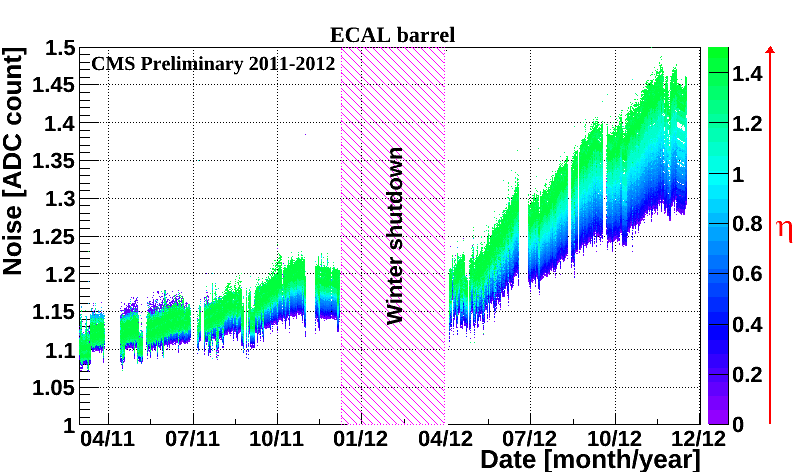
\includegraphics[width = 0.45\textwidth]{figures/ecal/EB_noise_ADC_counts_2011_2012.png}
  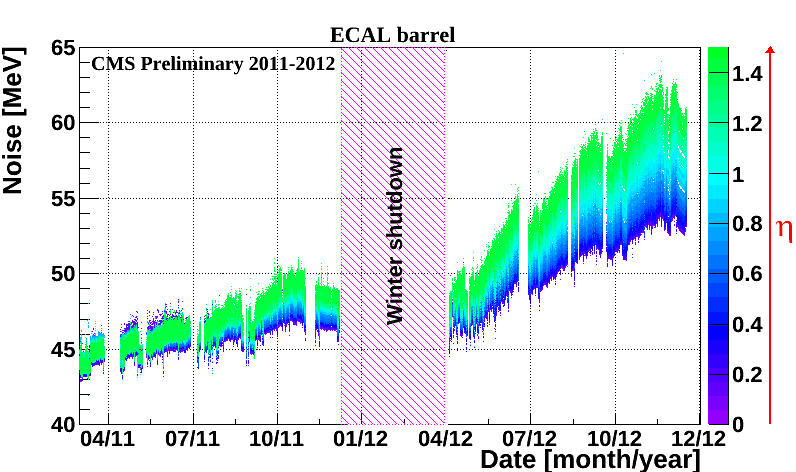
\includegraphics[width = 0.45\textwidth]{figures/ecal/EB_noise_MeV_2011_2012.png} \\
  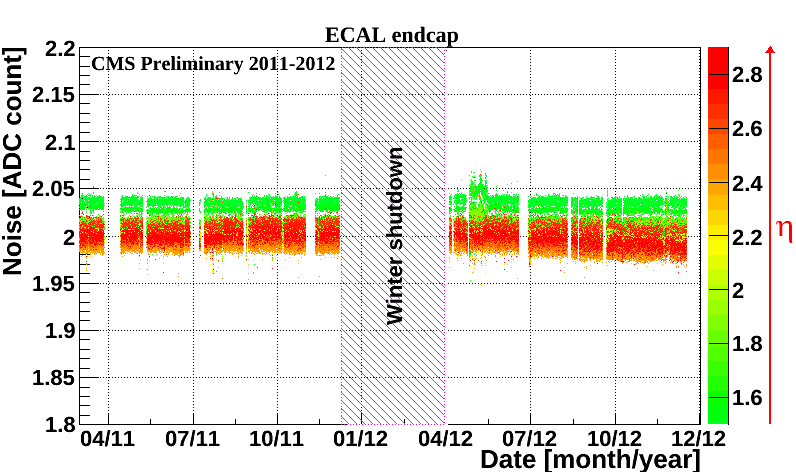
\includegraphics[width = 0.45\textwidth]{figures/ecal/EE_noise_ADC_counts_2011_2012.png}
  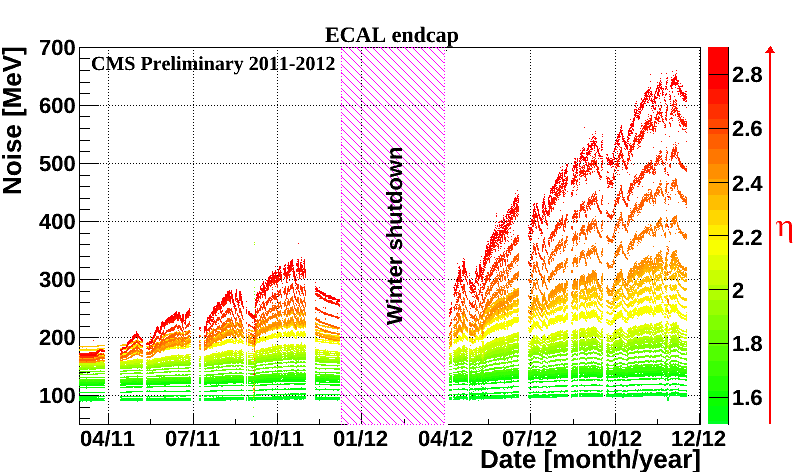
\includegraphics[width = 0.45\textwidth]{figures/ecal/EE_noise_MeV_2011_2012.png}
  \caption{Single channel noise measured on the pre-samples of the laser events taken during
    standard monitoring sequences in 2011 and 2012. The left plot shows the noise in ADC count prior the
    correction for the response loss measured with the laser system while the right one the noise in MeV
    after the correction. Top (bottom) plots inlcudes channels of the ECAL barrel (endcaps)~\cite{ecal_2012}.}
  \label{fig:ecal_noise}
\end{figure}

During 2015 and 2016 the calibration stream recorded events at a variable rate between 1 and 3 kHz with peaks of 20 kHz during
commisioning periods. The rate is kept under control by prescaling zero-bias events (whose rate is almost 40 MHz).

The loss of transparency occuring in the crystals increases the equivalent noise (expressed in GeV) since the
signal amplitude in ADC count is multiplied by the transparency correction derived with the laser system.
For this reason the events used in the intercalibration process
are required to have an energy above a thresholds ($E_{min}$) that takes into
account both the noise level and the loss of transparency and to have a transverse energy not grater then
$E_{min}/cosh(\eta) + 1 GeV$. This higher bound avoids that the energy sum used in the intercalibration is
biased along a certain $\phi$ direction by energetic deposit coming from hard scatterings which might not be
$\phi$-symmetric. The $E_{min}$ depends on the level of irradiation ad was set to $0.8$ GeV in 2015 and $0.9$ GeV in 2016, these
values were optimized to avoid noise induced distortions of the spectrum while keeping the amount of data needed
to derive an intercalibration close to that recorded in a typical LHC fill.
Selecting only depoists in a fixed energy window overestimates any response mis-calibration. This effect in taken into
account by introducing a scaling parameter ($k$) in the intercalibration formula to correct the ratio $\sumEt/\sumEtring$:
\[
  IC = \left( \frac{\sumEt}{\sumEtring}  \cdot \frac{1}{k} \right)^{-1}
\]
$IC$ is the correction factor to be applied to the original intercalibration coefficient in order to obtain the
new intercalibration and is computed for each one of the ECAL channels.
The $k$ parameter is estimated by multiplying the reconstructed energy of each hit by ten known
mis-calibration values ($m_{true} \in [0.9, 1.1]$), the observed mis-calibration is computed as:
\[
  m_{obs} = \frac{\sum E_T(m_{true})}{\sumEt}
\]
and the $k$ parameter is finally extracted as the slope of the linear fit to the distribution of $m_{obs}$ versus $m_{true}$
(Figure ??). The assumption of linearity 
The $k$ parameter depends on the shape of the $E_T$ spectrum so it is computed each time a set of intercalibration
is derived and for each ECAL channel independently, in this way variation of the spectrum induced by the different transparency
conditions are taken into account. Typical values for the $k$ parameter are within 2 and 2.5.

The statistical precision on the intercalibration values is estimeted by dividing the dataset by even and odd event number
and by computing the $IC$ for each channel with the two separate sub-dataset.
The $RMS$ of the crystals $(IC_{even}-IC_{odd})/(IC_{even}+IC_{odd})$ distribution divided by $\sqrt{2}$ is quoted as statistical
uncertainty on the $IC$ obtained with the full dataset (the uncertainty value is common for all crystals in the EB and EE).
Typically a new set of $IC$ is derived for each LHC fill (1-2 days) with a relative statistical uncertainty of about $0.4\%$.

\subsection{Energy calibration of the ECAL in 2015}
\label{sec:calib_2015}

After two years of long shutdown LHC resumed operation in 2015 with a higher beam energy 6.5 TeV (instead of 4 TeV) resulting
in 13 TeV of center of mass energy of the p-p collisions. The single channel response of the ECAL, although corrected
for the response variation measured with the laser system, has been corrected with a new set of intercalibration
derived combining the three intercalibration methods.

As explained in Section~\ref{sec:phisym} the $IC$ values derived with the $\Phi$-symmetry method are affected by
a large systematic uncertainty due to the presence of material in front of the ECAL, such effect cancels when taking
the ratio of two sets of $IC$ computed with data collected at different times. This cancellation however does not occur
when the two set of $IC$ are derived with collisions at a different center-of-mass energy.
The effect of the material on the $IC$ is clearly visible in Figure ??: the presence of support structures and services
absorbs part of the particle energy. This translates into a lower than average \sumEt, and conseguently higher $IC$ value,
for the ECAL crystals installed behind those structures. The material is however uniform along $\eta$ for crystals within 
the same tracker partitions (barrel and endcaps), so corrections for the impact of material are computed averaging
over $\eta$ the measured $IC$ values at same $\phi$ but for two regions in the EB ($|\eta|<1$ and $1<|\eta|<1.442$).
The $IC$ values are scaled for the average supermodule $IC$ and the correction for the $j-th$ $\phi$-row is defined as:
\[
C_j = \frac{1}{IC_{<\eta >}}
\]
The correction derived in this way are assumed to correct only for crystal-by-crystal variations introduced by the
presence of material in front of ECAL and not for real channel response variations.
The assumption is testet
comparing the correction values derived separately for $\eta <0$ ($C_j^+$) and $\eta > 0$ ($C_j^+$)
(Figure~\ref{fig:material_corrections})
and checking that the pull distribution $(C_j^+ - C_j^-)/\sqrt{\sigma_j^{+ 2}+\sigma_j^{- 2}}$
has a standard deviation equal to $1$ (Figure~\ref{fig:correction_pull}). This confirms that the observed variations
are independent of $\eta$ (in the two region defined above) within uncertainties while a channel mis-calibration
would appear as a systematic variation of the pull.
In total 720 correction values are computed (360 $\phi$-row for two $\eta$ regions) 
The correction computed in this way also correct for gaps in the $\phi$ direction present at the boundary of the ECAL barrel
supermodules (Figure ??). Crystals in supermodules installed in the positive and negative $\eta$ sides of the barrel
have opposite tilt angles, for this reason the effect of the gaps is on the last crystal of a supermodule for the positive
side while on the first one in negative side.
Gaps along $\eta$ are also present as shown in Figure ?? but are irrelevant when computing
the $IC$.

\begin{figure}[h!]
  \centering
  \includegraphics[width = 0.45\textwidth]{figures/ecal/corr_profile_2012_innerEB.pdf}
  \includegraphics[width = 0.45\textwidth]{figures/ecal/corr_profile_2015_innerEB.pdf}\\
  \includegraphics[width = 0.45\textwidth]{figures/ecal/corr_profile_2012_outerEB.pdf}
  \includegraphics[width = 0.45\textwidth]{figures/ecal/corr_profile_2015_outerEB.pdf}
  \caption{Material effect corrections for the barrel inner ($|\eta| < 1$, top row) and outer ($1 < |\eta| < 1.442$, bottom row)
    regions described in the text, the blue (red) curve refers to the negative (positive) $\eta$ side of the barrel.
    Plots on the left(right) side show the corrections for the 2012(2015) $IC$.
    Supermodules gaps affect the $IC$ of the first or last crystal in the supermodule if it is located on the negative or
    positive $\eta$ side respectively. The correction for gaps can be seen in plot as positive correction of about $6\%$
    every 20 $\phi$-rows while. The magnitude of the correction for material effect il larger for 13 TeV collisions (2015)
    than for 8 TeV ones, this can be clearly observed in crystals located behind the main tracker support structures located
    at the 10-th and 190-th $\phi$-rows. The correction for gaps at the supermodule boundaries are on the other end
  independent of the collisions energy since they only depend on the acceptance variation induced by the gaps.}
  \label{fig:material_corrections}
\end{figure}

\begin{figure}[h!]
  \centering
  \includegraphics[width = 0.45\textwidth]{figures/ecal/corr_pull_2012_innerEB.pdf}
  \includegraphics[width = 0.45\textwidth]{figures/ecal/corr_pull_2015_innerEB.pdf}\\
  \includegraphics[width = 0.45\textwidth]{figures/ecal/corr_pull_2012_outerEB.pdf}
  \includegraphics[width = 0.45\textwidth]{figures/ecal/corr_pull_2015_outerEB.pdf}
  \caption{Pull distribution of the correction difference between the positive and egative $\eta$ side of the ECAL barrel.
    Plots in the top and bottom row show the pull for inner ($|\eta| < 1$, top row) and outer ($1 < |\eta| < 1.442$
    respectively. Left (right) side refers to corrections for 2012 (2015) $IC$ set. Crystals located at supermodule
    boundaries are excluded from the pull since the gaps are, in principle, unrelated between the positive and negative
  barrel side.}
  \label{fig:correction_pull}
\end{figure}


The same material induced effects are observed in the endcaps but no way to factorize it from real channel-to-channel
variations has been found and a larger uncertainty has thus been attributed to the $IC$ values derived with $\Phi$-symmetry.

The corrected barrel $IC$ values are shown in Figure ??, the channel-by-channel ratio of the two $IC$ set (computed with
data from the last period of data-taking in 2012 and the first one in 2015) has been used to correct the intercalibration
derived by combining the three methods in 2012 in order to provide a new intercalibration for 2015. The $\eta$-ring
response variations has also been adjusted with the method described in Section~\ref{sec:minchia_la_calibrazione}.

To obtain the final channels intercalibration for EB channels the $IC$ values from the three methods are combined, the final values
for each channel is the weighed average of the three. The weight used for the combination is the uncertainty on the $IC$
measure dby each method and is estimated for each $\eta$-ring by computing the variance of the $IC$ difference for each
pair of methods. These variances are assumed to be to sum in quadrature of each method uncertainty consequently,
the precision of each intercalibration set is extracted by solving three simultaneous equations for the three the uncertainties.
The results on the uncertainties are reported if Figure~\ref{fig_ecal_ic_precision}. Taking advantage of the
small statistical uncertainty and the reduced impact of the material the $IC$ derived with $\Phi$-symmetry has the best precision
in all $\eta$-rings. The intercalibration with electrons precision is dominated by the statistical uncertainty which
is smaller at smaller $\eta$.

\begin{figure}[h!]
  \centering
  \includegraphics[width = 0.7\textwidth]{figures/ecal/ICs_precision.pdf}
  \caption{Residual miscalibration of the ECAL Barrel (EB) channel inter-calibration, as a function of pseudo-rapidity with the dataset recorded during 2015. The red points refer to the intercalibrations derived with Run1 data, extrapolated to 2015 using the laser monitoring system, and corrected using the $\phi$-symmetry of the low energy deposits in the 2015 dataset. The green points refer to intercalibration constants obtained using photons from $\pi_0\to\gamma\gamma$ decays, while the blue points to that obtained using electrons from W and Z decay .The black points represent the residual miscalibration of the combination of the three methods (weighted average). The precision of the $\Phi$-symmetry and $\pi_0$ calibrations is at the level of the systematic errors. The precision of the electron calibration is dominated by the statistical errors with the dataset recorded in 2015 (2.6 \fbinv). References: CMS DP 2013/007}
  \label{fig:ecal_ic_precision}
\end{figure}

In the endcaps only intercalibration values from $\Phi$-symmetry and electrons were available and they were combined
without weights.

The energy resolution achieved with final intercalibration, including the ring to ring
correction derivend with the method described above, is shown in Figure~\ref{fig:ecal_res_vs_eta}.
The resolution $\sigma_E/E$ is extracted from an unbinned likelihood fit to \Zee events,
using a Breit-Wigner function convolved with a Gaussian as description of the Z boson invariant mass peak.
The resolution is affected by the amount of material in front of the ECAL and is degraded in the vicinity of
the cracks along the $\eta$ direction between ECAL modules (indicated by the vertical lines in the plot)
The resolution, especially in the barrel, improves significantly after a dedicated calibration by using
the transported calibrations derived in 2012 and combining them with the calibrations obtained
from the 2015 CMS dataset (blue points),
compared to the prompt reconstruction using only the unmodified 2012 calibrations (black points). 
The resolution in the central barrel reaches the level achieved in Run1,
while int the endcaps the resolution is still significantly affected by the statistical precision of the calibration
(derived with a dataset equivalent to $2.6\fb$).

\begin{figure}[h!]
  \centering
  \includegraphics[width = 0.7\textwidth]{figures/ecal/EcalEnergyResolutionGolden.pdf}
  \includegraphics[width = 0.7\textwidth]{figures/ecal/EcalEnergyResolutionShowering.pdf}
  \caption{Relative electron (ECAL) energy resolution unfolded in bins of pseudo-rapidity $\eta$
    for the barrel and the endcaps \cite{ecal_dpg_2015}. Electrons from \Zee decays are used.
    The vertical dashed lines indicate module boundaries while the grey band around $\eta = 1.5$ denotes the transition
    between barrel and endcaps.
    The resolution is shown for low (left plot) and high (right plot) bremsstrahlung electrons,
    the categorization is based on the $R_9$ variable ($R9=E_{3x3}/E_{SC}$, where $E_{3x3}$ is the energy
    deposited in the most energetic crystal in the cluster and the 8 surrounding ones while $E_{SC}$ is the total
    supercluster energy as expressed in Equation~\ref{eq:sc_energy})}
  \label{fig:ecal_res_vs_eta}
\end{figure}

The residual differences between data and simulation
are due to the statistical uncertainties (endcaps) and other systematic effects described in \cite{run1_egamma}.
Part of these effects are variation of the response over time that are not corrected using the laser monitoring
system data. During 2016 thanks to a larger dataset these effects have been investigated in more details as
described in the next section.

\subsection{ECAL energy response monitoring in 2016}
Given the relative short break between the two data-taking periods (compared to the LS1)
the calibration obtained with data in 2015, corrected for the response variation
due to transparency gain observed with the laser system, was used as baseline
for the energy reconstruction during the 2016 data-taking period.
The energy reconstruction algorithm described in Section~\ref{sec:ecal_reco} was found to depend on both
the crystal-by-crystal noise level and signal shape used in the fitting procedure, thus a monitoring and prompt adjustment
of both quatities was develloped during the data-taking. The energy calibration process described in this section
is based on data reconstructed with the updated and time-dependent reconstruction. 

A drift over time of the energy scale was however observed during the year as variation of the Z boson
invariant mass peak in the di-electron spectrum, together with a constant worsening of the resolution.
As explained in Section~\ref{sec:laser}, the transparency variation observed with the laser system differs
from the one affecting the scintillation light collection by an exponetial factor $\alpha$.

The per-crystal $\alpha$ parameter can be measured using the same low energy particles from soft collisions
use for the $\Phi$-symmetry intercalibration method. The measurement is performed by minimizing the $\chi^2$:
\begin{equation}
  \chi^2 = \sum_{t=0}^n \left( \frac{F(t) \cdot \left(\frac{R(t)}{R(t_0)}\right)^{\Delta\alpha}}{\sigma_{F(t)}} \right)^2
\end{equation}
\label{eq:chi2_fit_alpha}

where $R(t)/R(t_0)$ is the relative response variation to laser light described in Section~\ref{sec:laser},
$F(t)$ is the ratio defined in Equation~\ref{eq:eflow_def} and $\sigma_{F(t)}$ is the uncertainty on $F(t)$.
The $F(t)$ ratio contains the same truncated transverse energy sum used to intercalibrate with the $\Phi$-symmetry method, thus
the $k$ parameter used to translate the obeserved mis-calibration into the real one is also applied here:
\begin{equation}
F(t) = \frac{ \frac{\sumEt(t)}{\sumEtEB(t)}  \cdot \frac{1}{k(t)}} { \frac{\sumEt(t_0)}{\sumEtEB(t_0)}  \cdot \frac{1}{k(t_0)}}
\end{equation}
\label{eq:eflow_def}
where \sumEt is the the same sum used for the intercalibration procedure while \sumEtEB is the sum over the chosen period of time
of all the transverse energy deposited in the EB.
Since the uncertainties on \sumEtEB and \sumEtring are both negligible with respect ot the crystal \sumEt,
the uncertainty $\sigma_{F(t)}$ is set to equal to the precision on the $IC$ estimated by dividing the data in each calibration
period $t$ in even and odd events (about $0.4\%$, see Section~\ref{sec:calib_2015}).

The $\chi^2$ (\ref{eq:chi2_fit_alpha}) is minimized with respect to the $\Delta\alpha$ parameter which is the difference
between the ``true'' crystal $\alpha$ and the average value used in the standard reconstruction. The \sumEtEB normalization
chosen to compensate for variations in the istantaneous luminosity or trigger rate, also absorbs variation common
to all crystals in the barrel, thus preventing the possibility of measuring a coherent variation of $\alpha$ among all crystals
in the ECAL barrel or a global scale variation of ECAL. The $F(t)$ variation over time together with the value of $1/LC(t)$
and the $F(t)$ derived with the fitted crystal $\alpha$ are shown in Figure~\ref{fig:eflow_examples} for two crystals
in the ECAL barrel.

\begin{figure}
  \centering
  \includegraphics[width = .45\textwidth]{figures/ecal/history_eb_good_BTCP.pdf}
  \includegraphics[width = 0.45\textwidth]{figures/ecal/history_eb_good_SIC.pdf}
  \caption{Example of $F(t)$ variation over time for two crystals in the ECAL barrel, produced by BTCP (left) and SIC (right).
    The open red dots are the $F(t)$ values obtain with the constant $\alpha$ value (reported as $\alpha_{db}$ in the figures),
    while the full red dots are the $F(t)$ values computed using the per-crystal $\alpha$ obtained from the fit described in the
    text (reported as $\alpha_{fit}$). The inverse of the correction for laser response variation is also shown (black full dots).
    For the BTCP crystal the $\alpha_{db}$ gives a stable response while the SIC crystal response varies up to $5\%$
    with respect the average ECAL barrel response. The corrected response is reported as closure test of the procedure.}
  \label{fig:eflow_examples}
\end{figure}


The fit results are shown in Figure~\ref{fig:alpha_fit}, the precision on the value of $\Delta\alpha$ extracted from the fit
varies between $1.8\%$ and $2\%$. The measured relative variation of the crystal-by-crystal $\alpha$ varies between
$\pm 20\%$ for the majority of the barrel crystals. A notable exception is rappresented by crystals produced by the SIC company
for which an  $\alpha$ value of one was measured at the pre-installation beam tests, the value extracted from the fit
with 2016 data is on average $1.4$. The same fit has been performed also for crystals in the ECAL endcaps but due to the
different injection point of the laser light, which makes the response to laser and scintillation light more similar, and
the convolved effect of the VPT aging the uncertainty is larger ($10\%$) and the results compatible with the constant $\alpha$
used in the standard reconstruction.

\begin{figure}[h!]
  \centering
  \includegraphics[width = 0.45\textwidth]{figures/ecal/EB_delta_alphas.pdf}
  \includegraphics[width = 0.45\textwidth]{figures/ecal/EB_chi2.pdf} \\
  \includegraphics[width = 0.7\textwidth]{figures/ecal/mapEB_delta_alpha.pdf}
  \caption{Measured $\Delta\alpha$ values for crystals in the barrel (top left) and fit $\chi^2$ (top left),
    each distribution is normalized to its area.
    The $\Delta\alpha$ values are reported as relative variations from the $\alpha_{db}$ value of 1.52(1) used
    in the energy reconstruction for BTCP(SIC) crystals.
    The bottom plot shows the distribution of the relative $\Delta\alpha$ in the $\eta$-$\phi$ plane (where instead
    of the absolute $\eta$ and $\phi$ coordinates the discrete crystal indices $i\eta$, $i\phi$ are used).
    The map highlights the SIC crystals (red region at high $|\eta|$) and the block structures described in the text.}
  \label{fig:alpha_fit}
\end{figure}

The measured $\Delta\alpha$ values present block patterns in the $\eta$-$\phi$ plane (Figure~\ref{fig:alpha_fit} bottom)
compatible with the granularity of the PN sensors described in the Section~\ref{laser}, with a variation of $\alpha$
within such blocks much smaller than the block to block variations. The observed behaviour is compatible with a linear drift
of the PN electronics response and thus unrelated to the crystal $\alpha$.
The effect has been investigated also using electron from Z and W boson decays, highlighting the same block pattern
and an overall coherent drift of the barrel scale, to which the $F(t)$ is insensibile for the reason explained above.
For this reason an effective correction to each PN block response has been prefered for the final 2016 erconstruction.
The correction was derived using the measured average $\alpha$ value of $1.4$ for the SIC crystals and by performing
a linear fit to the $E/p$ peak variation as a funtion of time with a granularity of one LHC fill. An example fit for
one PN block is shown in Figure~\ref{fig:pn_fit}, the measured drifts are equivalent to a scale variation
between $0.1\% / 30 days$ and $0.2\% / 30 days$ depending on the average $|\eta|$ of the PN block, with larger drift
at larger $|\eta|$.

\begin{figure}[h!]
  \centering
  \includegraphics[width = .7\textwidth]{figures/ecal/EoP_PNfit_example.pdf}
  \caption{Example fit of a region of 200 crystals monitored by the same PN diode. The $p1$ parameter rappresent
    the slope of the linear fit and is equivalent to $0.18\% / 30 days$}
  \label{fig:pn_fit}
\end{figure}


The final energy scale stability and resolution are shown in Figure~\ref{final_2016}: although a good stability on
the energy scale is achived (better than $0.5\%$) the resolution still get worse during the data-taking period, underlining
a residual channel-to-channel response variation.

\begin{figure}[h!]
  \centering
  \includegraphics[width = 0.45\textwidth]{figures/ecal/scale-Cal_Mar2017_PNcorr_v2-EB.pdf}
  \includegraphics[width = 0.45\textwidth]{figures/ecal/resolution-Cal_Mar2017_PNcorr_v2-EB.pdf}
  \caption{ECAL energy scale and resolution stability during the 2016 data-taking period. With the
    optimized calibration discussed in the text (black) and the calibration of 2015 (red).
    The energy scale (resulution) stability is displayed on the left (right) and is measured with \Zee events in
    which both electrons are detected in the barrel. The peak estimator is the median of the Z invariant mass peak, while
    the resolution is estimated as the minimal symmetric interval including $68\%$ of the events around the peak and is
    reported in the plot in fraction of the estimated Z boson mass value in each period.}
  \label{fig:final_2016}
\end{figure}


\section{Summary}
The ECAL energy response is subject to eveloution over time mainly due to the loss of transparency following irradiation.
Although a powerful monitoring system based on the injection of laser light allows to correct for the transparency loss,
a residual mis-calibration affects the energy measurement. A new ECAl calibration was derived in 2015 after a 2 year long
LHC shutdown combining the three intercalibration methods developped during the first collison period of LHC,
resulting in an energy resolution at the level fo $1\%$ for non showering electrons in the barrel and $2.5\%$ in the
endcaps comparable to that achived during the first running period of LHC.
During 2016 the time evolution of the detector response was studied in great detail, a method to measure a
per-crystal $\alpha$ parameter was successfully implemented.
The same study lead to the observation of unexpected drift in
the laser monitoring electronics which were corrected using electrons from Z and W boson decays. The procedure defined in
2016 will serve as a roadmap for future energy calibration of the ECAL.
    
    
  
  
  

\clearpage\chapter{Search for resonances decaying to two photons}
\label{chapter:diphotons}

In this chapter the search for resonant BSM prodoction of photons pairs is presented.
First the the analysis approach and event selections optimization are described, then
the statistical analysis and finally the results.

The analysis has been optimized for searches performed on data collected from proton-proton
collisions at a center of mass energy of 13 TeV. The optimization has been performed with
data collected during 2015 corresponding to an integrated luminosity of \lumififBon.

\section{Data samples}
\label{sec:diphotons_data_samples}
The search is perform in data collected by the CMS experiment during the year 2016. The total
integrated luminosity is \lumisix. Data are reconstructed witha detector calibration optimized
for the 2016 p-p collision datataking period.

The events were recorded with a trigger designed to select events containing a pair of
energetic photons with $E_T > 60$ GeV. The energy of each photon candidate is computed as
the sum of the energy measured by ECAL and HCAL and trigger selections require
the energy measured in HCAL to be less than $10(15)\%$ of that measured by ECAL for candidates
in the calorimeter barrel(endcap) region.

The trigger is found to be fully efficient for photons with $\pt > 75$ GeV and so an offline
selection is applied to select these events.

Together with the main analysis trigger another one is used to select electrons from \Zee decays.
The \Zee is the primary control sample of the analysis and events compatible with this process
are recorded with a single electron trigger that selects events with at least one electron of
$\pt > 27$ GeV and $|\eta| < 2.1$. Tight isolation and identification critaria are applied at trigger
level to maintain a rate compatible with the DAQ capabilities.
\Zee events are used to measure the final photon selection efficiency so the single electron trigger
is preferred over a double electron one, since in this way an unbiased set of electrons can be
constructed from those coming from \Zee decays that did not triggered the event acquisition.

\section{Monte Carlo simulated samples}
The Monte Carlo simulation of the CMS detector and 13 TeV p-p collisions is used. The simulation
takes into account both the pileup generated by concurrent interactions and the presence of
signals in the detector coming from collisions in other bunch crossing. Events in the simulated samples
are re-weighted to match the pileup energy density distribution measured in data.

\subsection{Resonant signal simulation}
\RS gravitons are chosen as a reference for the spin-2 resonance search. SM-like Higgs bosons of high mass and
fixed widths are used for the spin-0 case.
A set of simulation samples is used to model the detector response to resonant production of two photons.
Such samples are generated with PYTHIA8 in the mass range $500 < \mgg < 7000$ GeV in steps of 250 GeV for
masses below 4 TeV and 500 GeV above it. An additional set of samples without simulation of the detector
response are used to model the signal spectrum and the acceptance of the kinematic selections.
Three relative width hypothesis $\Gamma/\mgg$ are taken as benchmarks: $0.1\%$, $5\%$ and $5.6\%$ which,
in the case of \RS gravitons, correspond to a $k/M_{planck}$ of $0.01$, $0.1$, $0.2$ respectively.

\subsection{Standard model diphoton production simulation}
Even though the shape and yield of SM non-resonant diphoton production are measured with fit to the data,
simulated samples of the background processes are used for analysis optimization. A set of QCD induced
$\gamma+jet$ events generated with PYTHIA8 is used to optimize the photon identification selections.
The events are produced in several invariant mass bins in order to have a significant amount of photons and
jets over the whole $p_T$ spectrum.

\subsection{Drell-Yan production of electron-positron pairs}
Finally a set of Drell-Yan events ($Z/\gamma* \to e^{+}e^{-}$) is generated with aMC@NLO and is
used to derive data to simulation scale factors for the selections efficiency.

\section{Events selection}
Two measurement are needed to build the invariant mass of the diphoton system: the energy of the
photons and the interaction vertex position. The former is performed with the ECAL as described in
Section ??? while the latter is reconstructed with tracks produced in the interaction against which
the diphoton system recoils. Additional information from the tracker and the HCAL are used to discriminate
genuine photon candidates from QCD jets.
In the following paragraphs the vertex and photon identification algorithms are presented.

\subsection{Vertex identification}
The standard CMS reconstruction identify the primary interaction vertex as the one withing each
bunch crossing that as the largest $\Sigma p_T^2$ (where the sum runs over all the charged particles
coming from the vertex). The method is not fully efficient for diphoton events since the two neutral
particles carry a significant amount of the transverse energy.
A dedicated boosted decision tree regression has been trained in the context of the search for the
Higgs boson decaying into two photons. Inputs to the regression are the $\Sigma p_T^2$ and
other quantities related to the $p_T$ balance between the diphoton system and the charged particles.
Using this method the interaction vertex is correctly assigned for about $90\%$ of the signal events.

\subsection{Kinematic selections and event categorization}
\label{subsec:event_cats}
Photons candidates are reconstructed from energy deposit in the ECAL with no associated track.
A set of kinematic selection is applied to avoid detector inefficiencies and shaping of the mass
spectrum due to trigger level selections:
\begin{itemize}
\item The transverse momentum of each candidate had to be above $75$ GeV.
\item The absolute value of the pseudorapidity of the supercluster (\absScEta) of both
candidates had to be below $\absScEta < 2.5$ and not between $1.444 < \absScEta < 1.566$,
due to the geometric acceptance of the ECAL.
\item To avoid a distortion of the background shape due to the transverse momentum
cut, the minimum invariant mass of the diphoton pair had to be $230$ GeV, when
both photons were detected in the ECAL barrel region (EB, $\absScEta < 1.444$). If one photon candidate
was detected in the endcap region (EE, $\absScEta > 1.566$), the minimum invariant mass
had to be $320$ GeV.
\end{itemize}

If more then one pair of photons satisfies the kinematic selection ($1\%$ of all the events) the pair
with the highest scalar sum of transverse momentum $p_T^{\gamma\gamma}$ is chosen.

The events are split into two categories accordingly to the topology of the photon system in relation
with the ECAL segmentation:
\begin{itemize}
\item barrel-barrel (EBEB): both photons are detected in the ECAL barrel region $\absScEta < 1.444$.
\item barrel-endcap (EBEE): one photon is detected in the ECAL barrel region $\absScEta < 1.444$ the other
  in one of the endcaps $1.566 < \absScEta < 2.5$.
\end{itemize}

The EEEE category (both photons detected in the endcaps regions) is not considered for the analysis
since only few percent of the benchmark signal events fall in this category and conversely the SM
background is considerably higher than in the other categories.

\subsection{Photon identification}
Energetic neutral pions found in QCD jets has a similar signature since they decay into two collimated
photons. A dedicated set of selection is applied to each photon candidate in the analysis to select a pure
sample of diphotons events. These criteria were optimized for photons with high transverse
momentum and based on the following variables:

\begin{itemize}  
\item \chIso: the scalar sum of the transverse momenta of the particle flow charged hadron
candidates, which are assigned to the chosen primary vertex. Only candidate
within a radius of $\DeltaR < 0.3$ from the photon in the $\eta$ - $\phi$ plane, which is
defined as:
\[
\DeltaR = \sqrt{(\eta_\gamma-\eta_{cand})^2 + (\phi_\gamma-\phi_{cand})^2}
  \]
are considered.

\item \phoIso: the scalar sum of the transverse energies of the particle flow photon candi-
  dates for which $\DeltaR < 0.3$.
  
\item \hoe: ratio of the energy measured in the HCAL and ECAL.

\item \sieie: the weighted spatial second order moment of the photon candidate in the
  $\eta$-direction, computed as:
  \[
\sieie = \sqrt{\frac{\Sigma_{i}{}}{}}
\]

\item Conversion safe electron veto, to reject electrons.

\end{itemize}

Particle flow charged particles or photons sharing part of their energy with the photon candidates
are excluded from the \chIso and \phoIso sum. 

The thresholds of the identification variables were optimized to give an efficiency flat as a function
of the mass of the diphoton pair, the chosen working point correspond to an efficiency of $90(85)\%$ for
photons in the EB(EE).
The \phoIso distribution is found to depend on the event pile-up and the $p_T$ of the
photon candidate. These dependencies leads to a variation of the selection efficiency with time and also
for different values of \mgg. In order to keep a flat effiency a correction is used, its expression is:
\[
  \phoIso^{corr} = \phoIso - \kappa\cdot p_T - A \cdot \rho + \alpha
\]

where $p_T$ is the transverse momentum of the photon candidate, $\rho$ is the event pile-up energy density.
The values of $A$ and $\kappa$ are chosen such to keep the $90\%$ quantile of the distribution at a constant
value as a function of $\rho$ and $p_T$, while the $\alpha$ parameter is used to adjust the distribution such
that the bulk of the corrected isolation distribution for signal photons peaks at zero.

For very energetic photons the ECAL readout electronics can saturate. In such a case the shower shape variable
\sieie is distorted, hence a different selection value is set for this identification variable in case of saturation.

\subsection{Selection efficiency measurement}
The efficiency of the photon identification described in the previous chapter is measured with data
using the \Zee control sample. The measurement of the selection efficiency in data is then
compared to the one measured in the simulation and in case of discrepancy the signal normalization
derived from the simulation is corrected for the measured scale factor.

The efficiency is measured with a tag-and-probe technique exploting the well known Z decay to electrons.
For this study the response of the ECAL and HCAL is assumed to be identical for electrons and photons.
The tag-and-probe method is used both for the data and simulation mesurement, the \Zee control sample
in data is selected using events recorded with a single electron trigger (???). Di-electron candidates
are further filtered with an invariant mass selection ($70 < \mee < 110$ GeV) centered around the Z mass peak,
the invariant mass window is applied also to the simulated events.

The method then requires one of the two electrons (the ``tag'') coming from the Z boson to pass a very tight selection
(this tight working point is developped by a dedicated group within CMS and provide high purity electrons
with an effiency of $70\%$).
The second electron is required to pass a loose identification and is assumed to be an unbiased
with respect the variables being studied (the ``probe''). The photon selection efficiency is studied using
this unbiased sample inverting the electron veto request.

Since the chosen trigger requires the electron to be within $\absScEta < 2.1$ the tag electron
is required to be within this region too. The efficiency is studied as a function of the electron $p_T$
and the event pile-up energy density $\rho$.

The data events are fitted
simultaneously for passing and failing probes with a signal plus background model.
The signal is modeled by the Z lineshape as obtained from a QCD NLO (POWHEG)
generator convolved with a Gaussian, while the background is modeled by an exponential function. As
the choice of the fit model is one of the dominating systematics, different models were
studied to assess it [???]. A simple cut-and-count method is applied for the simulation sample
since the non resonant $pp \to \gamma^* \to e^+e^-$ events are discarded with MC truth information.

FIGURE!

\section{Photon energy scale and resolution corrections}
The detector simulation takes into account the effects of pilu-up, detector noise and response variation.
The pile-up distribution is then reweighted to match the one in data as explained in Sec~\ref{sec:diphotons_data_samples}.
The detector noise and response variation instead varies over the datataking period and so a discrepancy
in the energy response of the ECAL may arise between data and simulation since in the latter no time evolution
of the detector conditions is simulated. The effect of this discrepancy translate in shift of the energy
scale in data with respect to the MC simulation, furthermore any residual mis-calibration of the detector
is not simulated and thus the energy resolution in data is worse than in the MC simuation.
These two effects are corrected on one hand
scaling the photon energy (after being corrected with the method described in ???) in data events
in order to correct the time dependent scale variations and match the energy scale of the simulation and,
on the other hand, by smearing the energy in simulated events to match the resolution observed in data.

The time-dependent scale corrections and the smearing are derived with the \Zee control sample.
Again since the energy for both photons and electrons is primarly reconstructed from the ECAL, electrons
are used as a proxy of photons.

The corrections are derived in two steps: in the first, the energy scale is corrected by
adjusting the scale in data to match the simulation prediction. The \Zee invariant mass peak is fitted with
a Breit-Wigner function convolved with a crystal ball (CB) function describing, respectively,
the theoretical signal line shape of the Z-boson and the detector response.
The parameters of the Breit-Wigner function for the Z boson are taken from the Particle
Data Group (PDG) [8]: $m_Z = 91.1876$ GeV and $\Gamma_Z = 2.4952$ GeV.
By fitting the distribution in data and MC simulation separately, the energy scale offset can be extracted.

Different systematic behaviors of the mean of the CB function ($\Delta_m$) as a function of time and the
pseudorapidity can be observed. As a result, run dependent energy corrections are
necessary to correct for the energy scale variations during data-taking. The energy scale
correction ($\Delta P$) is defined as the relative shift in mass between data and MC prediction:
\[
  \Delta P = \frac{\Delta m_{data} - \Delta m_{simulation}}{m_Z}
\]

After the $\Delta P$ correction is applied, a stable behavior of $\Delta m$ over time within
0.1 GeV is observed.

In the second step, the residual difference between the observed and predicted electron
energy is assessed by maximizing the likelihood between the smeared MC distribution and the data.

The smearing of the MC distribution is performed by multiplying \scE distribution by a
Gaussian distribution, centered at $1 + \Delta P$ and with resolution $\Delta C$.
The resolution $\Delta C$ denotes the additional constant term of the energy resolution which
is added to the MC prediction.

The additional constant term needed to match the energy reasolution measured with data varies as a function
of \scEta, as the scale correction, but it also different between electrons that showers in the tracker volume
and those that don't.
The \rnine variable is used to discriminate between showering and non-showering electrons: this variables is used
instead of others since can also be applied to dfiscriminate between converted and un-converted photons and
so is suitable to mantain the analogy between the analysis object (photons) and the control sample ones (electrons).
Thus maximum likelihood fit is performed in eight categories: four \scEta regions times two \rnine categories.

The comparison between the predicted and observed dielectron invariant mass spectrum around the Z boson peak,
for events passing the analysis selection (with inverted electron veto) and after all energy corrections have been applied
is reported if Fig.~???.

Finally the linearity of the ECAL energy response is studied using Z bosons with high transverse momentum
decaying to electrons. This technique allows to test the linearity for transverse energies up to 150(100) GeV in
the EB(EE) region.
The linearity of the response is assessed by comparing the peak position of the
reconstructed Z mass measured in data and simulation as a function of $H_T = E_{T_1}^2 + E_{T_1}^2$, where
$E_{T_1,2}^2$ are the transverse energies of the two electrons.

For electrons detected in the barrel part of the detector, the energy scale corrections
were observed to be stable within $0.4\%$. Electrons detected in the endcap region of the
detector were found to provide a stability of better than $0.8\%$. More information can be
found in Ref.~???. A final $1\%$ uncertainty on the energy scale stability is assigned.

\section{Statistical interpretation of the results}
\label{sec:results}

This section presents the statistical technique used to interpret the analysis results.
The goal of the statistical analysis is to define a compatibility between the observed dataset
with the predicted standard model only and standard model background plus signal hypothesis.
Where no deviation from the standard model prediction is found results are interpreted in terms
of modified frequentist upper limits on the signal process cross-section.

First the signal plus background maximum likelihood fit to data is presented, then the signal and
background model derivation are described. The last part of the chapter is dedicated to the presentation of
the results of the hypothesis test.

\subsection{Signal plus background maximum likelihood fit to data}
A test statistic is build in order to test the different signal hypothesis, the underling likelihood
is defined as:
\begin{equation}
  \label{eq:likelihood}
  L(\mu, \theta) = \prod_{i\in Events}\Big[\mu\cdot S(\mgg^{i}|\theta_S) + B(\mgg^{i}|\theta_B)\Big]
  \cdot Poisson(N_{events}|N_B+\mu\cdot N_S)
\end{equation}

In this formula, $S$ and $B$ denote the signal and standard model background shape respectively. Both
models are $p.d.f$ that depends on \mgg and on nuissance parameters ($\theta$) that rappresent the systematic uncertainties.

The selected events are split in two categories as described in Sec.~\ref{subsec:event_cats}.
Thus two different likelihood are built: each categories has different nuissance parameters, signal and background shapes,
while the signal strengh $\mu $ is a common parameter.
A simultaneous fit to the data in the two category is performed.

\subsection{Background parametrization}
\label{subsec:background}
The background parametrization is extracted from a fit to the data performed separatelly for the two analysis
categories. The fit is performed assuming the absence of any signal, so the signal strengh $\mu$ is set
to zero in the likelihood~\ref{eq:likelihood}.
The choice of a data-driven techniques to define the background shape eliminates the need of high order
QCD calculation for simulated samples and also a precise knowledge of the background processes ratios.

A parametric form is chosen out of an arbitrary set of possible function.
To ensure that the particular choice of the functional form does not introduce any biases in the
background shape prediction, the accurancy of the chosen function is evaluated with the following
procedure:




\clearpage\providecommand{\sixbysix}{\ensuremath{6\times 6\mathrm{~cm}^{2}}\xspace}
\providecommand{\threebythree}{\ensuremath{3\times 3\mathrm{~cm}^{2}}\xspace}
\providecommand{\twobytwo}{\ensuremath{2\times 2\mathrm{~cm}^{2}}\xspace}
\providecommand{\onebyone}{\ensuremath{1\times 1\mathrm{~cm}^{2}}\xspace}

\chapter{The HL-LHC upgrade of CMS}
\label{chapter:cms_upgrade}

In this chapter the upgrade of the LHC complex is briefly introduced in Section~\ref{upgrade_lhc}
underlining the physics goal and the expected performace of the machine. The CMS experiment is already planning
a series of upgrades, most of which will be installed during LS3 (Figure~\ref{fig:lhc_plan}).
The overall goal of the CMS upgrade is introduced in  while
further details on the upgrade of the CMS ECAL are reported in the rest of the chapter.
The ECAL upgrade mainly concerns the read-out electronics and trigger system, these are introduced in Section ??
while in Section ??.

\section{High Luminosity LHC}
\label{upgrade_lhc}

The main objective of the High Luminosity LHC (HL-LHC) upgrade [9] of the LHC accelerator complex
is to make precise measurements of the Higgs boson couplings, the standard model and provide a very
large dataset ($3000\fbinv$) for new physics searches.
The design include a substantial upgrade of the accelerator complex with the goal of reaching
a peak luminosity of $7.5\times10^{34} cm^{-2}s^{-1}$ (roughly four times as mush as the current value)
The integrated luminosity will about ten times the expected luminosity of the first twelve
years of the LHC.
The timeline of LHC and HL-LHC operation is sketched in Figure~\ref{fig:lhc_plan}, showing the planned
evolution of proton beam intensity through the remaining LHC operating periods (Run 2 and Run 3)
and the HL-LHC operating period following the upgrade of the accelerator complex in LS3.
%The two periods of operation are termed Phase-1 (LHC) and Phase-2 (HL-LHC).

The peak luminosity will be achieved by increasing the beams intensities and by squeezing more the two beams at the
interaction points. This will lead to a higher number of collisions occuring within the same bunch crossing, the
average number of collisions will increase from 40-60 of LHC to 140-200 at HL-LHC.
The ability of the detectors (ATLAS and CMS) in assagning particles to the correct collision will worsen with the
increased instantaneous luminosity expetially for energy deposits in the calorimeters.


\section{HL-LHC upgrade of CMS}
\label{upgrade_cms}
The CMS detector will be upgraded to match the operation environment of HL-LHC in order to fully exploit the
larger dataset delivered by the accelerator complex.
The major points are
the replacement of the entire calorimeters system in the endcaps to cope with the expected level of radiation
of HL-LHC (more than $1.5\times10^{15} n_{eq}/cm^{2}$ in the parts closer to the beam line),
the complete replacement of the Level-1 trigger and the proposed installation of a new detector to measure the
time of charged particles with a precision of about $30 ps$. These three major points also drives upgrades of
the other existing components: the upgrade of the Level-1 trigger will profit from an extended
muon system coverage up to $|\eta| = 2.8$, new tracker system cabable of providing information at
Level-1 and calorimeter system electronics upgraded to match the trigger rate allowed by the Level-1.
The completely new calorimenter system in the endcaps will provide longitudinal shower development which will
in turn improve descimination between energy deposits coming from different collisions.
Finally the time information extracted with the new system will be matched by those of the ECAL barrel and the new
endcap calorimeter. The ECAL si expected to provide a time information on electromagnetic showers
with a precision of $30 ps$ for energies above few tens of GeV.

\section{The ECAL barrel upgrade}
The primary technical motivation for the ECAL barrel (EB) upgrade is the trigger requirement for
an increase of the trigger latency from about $4\mu$s in the current system [4] to a maximum of $12.5\mu$s,
and a Level-1 trigger rate of up to 750 kHz compared to the current 100 kHz.
The EB electronics Front End (FE) card and all the read-out electronics will be replaced to
meet these requirements. The current configuration provides trigger information to the Level-1
with a granularity of five-by-five crystals, the upgraded system will have a single crystal granularity
enhanching event selection based on isolation information at trigger level which will in turn allow
to set lower thresholds on the transverse energy of the candidate particles.

The foreseen upgraded FE electronics will also provide a shape discrimination between
signal compatible with an electromagnetic shower and those originated from hadronic interaction (``spikes'') in
the photodetector (APD) which have a narrower shape. The increased Level-1 granularity of a single crystals
will also improve the rejection of such events at trigger level.
The shape discrimination is made possible by a shorter signal shaping performed by the amplification chain
coupled with a signal sampling frequency of 160 MHz (four times the current). The increased sampling
frequency is also the key upgrade to provide a time measurement at the $30 ps$ level (Section ??) and
is limited by overall CMS constrain on data transfer bandwidth and power consumption.

% \subsection{The ECAL timing performance}
% To assess the timing capabilities of the ECAL a series of test beams have been carried out during the R\&D phase.
% The test beam goal is to first measure the intrinsic time resolution achievable with \PbWO crystals and
% APD system and at a second stage verify the performance with the sampling frequency of 160MHz.

\subsection{The current ECAL timing performances}
The time of an electromagnetic shower in the ECAL is defined as the time at which the signal generated
in the APDs reachs its maximum amplitude. The method to extract this information for the digitized signal
shape is described in \cite{ecal_time_reco}. The time of the maximum $T_{max}$ is estimated with each
available pair of samples (up to nine) as:
\[
T_{max, i} = T_i - T(R_i)
\]
where $i$ is the $i-th$ sample, $T_i$ is acquisition time of the $i-th$ sample and $T(R_i)$ is the time
corresponding to the amplitude ratio $R_i = A_i/A_{i+1}$ and is extracted from a parametrization whose parameters
were measured in a test beam prior the installation of CMS. The error ($\sigma_i$) on each $T_{max, i}$ is estimated as
the product of the derivative of the $T(R)$ function and the uncertainty on $R_i$ which is the sum in quadrature
of three components: noise fluctuations in each sample, uncertainty on the pedestal value subtracted from the measured amplitued
and trunction occuring during the 12 bit digitization of the amplitude.
For signal syncronized with the LHC bunch crossing only four or five of the nine possible amplitude
ratios are used, samples with very small amplitude are discarded. The unique signal time is computed
as the weighted average of the  $T_{max, i}$:
\[
  T_{max} = \frac{\sum_i T_{max, i}/\sigma_i^2}{\sum 1/\sigma_i^2}
\]
and the its error as:
\[
  \frac{1}{\sigma_{T_{max}}^2} = \sum_i\frac{1}{\sigma_i^2}
\]

The time resolution can be parametrized as:
\begin{equation}
  \sigma^2(t) = \left( \frac{N\cdot\sigma_n}{A} \right)^2 + \left( \frac{S}{\sqrt{A}} \right)^2 + C^2  
\end{equation}
\label{eq:general_time_res}

where A is the measured signal amplitude, $\sigma_n$ is the RMS of the noise for each sample and
N, S, C represent the noise, stochastic, and constant term coefficients, respectively.
The stochastic term S is related to fluctuations in the colletion times of scintillation photons due to
the finite time their emission.

% It was verified in \cite{ecal_time_reco} to have a negligible impact on
% the time resolution expetially when looking at the time difference for two crystals hit by the same electromagnetic
% shower . 

The time performance of the ECAL has been estimated both during the pre-installation test beam \cite{ecal_time_reco}
and with data collected during the 8 TeV operation of LHC \cite{delRe_time_ecal}.
In the test beam measurement the resolution was extracted from the time difference between the two most energetic crystals
af the same electromagnetic shower, in this configuration the stochastich term that appears in Equation~\ref{eq:general_time_res}
can be neglected since shower flactuation effects cancels out in the difference, Equation~\ref{eq:general_time_res} thus becomes:
\begin{equation}
  \sigma^2(t_1 - t_2) = \left( \frac{N\cdot\sigma_n}{A_{eff}} \right)^2 + 2 \cdot C^2
\end{equation}
\label{eq:ecal_time_res}
Where $A_{eff} = A_1A_2/\sqrt{A_1^2+A_2^2}$ and $t_{1,2}$, $A_{1,2}$ refers to the times and amplitudes measured by the two crystals. 
The time resolution $\sigma(t_1-t_2)$ was estimated with a gaussian fit to the time difference.
The results obtained in the analysis report a constant term of $20 \pm 4$ ps which, together with a noise term $N = 35.1\pm 0.2$ ns,
gives and expected time resolution better than 100 ps for energy deposits greater than 20 GeV in the barrel.

The prediction was tested wih data collected during 2011 and 2012 from CMS. With collisions events it is possible to
test the performance of the whole system including the clock distribution. \Zee events where used in \cite{delRe_time_ecal}
the results show a good performance when measuring the time difference for channels belonging to the same readout unit while
an increasingly poorer performance for channels in different readout units but same shower and channels belonging to
the two different superclusters in \Zee events (Figure~\ref{fig:ecal_runI_time}).

\begin{figure}[h!]
  \centering
  \includegraphics[width = 0.45\textwidth]{figures/upgrade/t_res_sameRO.pdf}
  \includegraphics[width = 0.45\textwidth]{figures/upgrade/t_res_diffRO.pdf}\\
  \includegraphics[width = 0.5\textwidth]{figures/upgrade/ecal_resol_Z.pdf}
  \caption{Resolution of time difference between the two most energetic crystals of an ECAL cluster as a function of the
    effective amplitude $A_{eff}$, normalized to the noise in the ECAL Barrel for 2011+2012 data,
    for crystals belonging to the same readout unit (top left), different readout unit (top right) and the two most
    energetic crystals in each of the superclusters generated by electron from \Zee decays (bottom).
    For electrons from Z boson decays the time of each crystals is corrected for the time of flight from the common
  interaction vertex.}
  \label{fig:ecal_runI_time}
\end{figure}

These results were interpreted to be due to time jitter introduced by the clock distribution system and not corrected by
the calibration performed with low energy deposits. The clock stability has been measured in 2016 using laser monitoring data
and while the time resolution constant term is found to be below $40 ps$ even for crystals belonging to different readout unit,
instabilities of the clock syncronization at the level of $100 ps$ were observed over the course of few days. The
observed effect is in agreement with the constant term measured using \Zee events that are collected over a long period of time.

\subsection{Test beam results with HL-LHC electronics}
During 2015 and 2016 a series of tests with electron beam were performed to evaluate the time performance
of the \PbWO crystal plus APDs photodetectors system (2015 beam test, Section~\ref{sec:tb_2015})
and that of the proposed HL-LHC ECAL electronics (2016 beam test, ??).
The tests differ from the ones conducted before the CMS installation since the time of the electron measured by the
crystal is compared to an external reference provided by a multi-channel-plate based detector (MCP) instead of to an adiacent
crystal hit by the some shower.

\subsubsection{Test beam setup}
\label{sec:tb_2015}
The first test was conducted in 2015 at the CERN SPS north area with a tunable beam of electrons with energies between 20 and 250 GeV.
The electron beam is a secondary beam created from the primary proton beam, extracted from the SPS, using a conveter.
The primary beam hits a metallic target producing a variety of particles that are selected through a system of magnets, collimators
and additional targets. The beam line used for the tests can reach a electron purity of $99\%$ and can also be
configured to provide a equally pure pion beam to study ``spikes'' in the APDs.
The beam in the SPS is composed of several bunches that are extracted in an interval of 4-5 s every 14-48 s depending on the
SPS cycle configuration. The extraction line is configured in a way to destroy the bunch scheme of the SPS beam in order
to provide a uniform and less intense beam to the test area.
The energy of the secondary beams of electrons, positron, muons and charged pions can be selected within the 10 to 400 GeV
range. 

The experimental setup included a $5\times 5$ \PbWO crystal matrix identical to those installed in the ECAL barrel,
with two APDs glued at the back (A schematic view of the setup is shown in Figure~\ref{fig:tb_setup}.
The APDs signals were amplified with the same $CR-RC$ circuit installed in the current ECAL
supermodules, the shaping time for some of the channels was set to 21.5 ns (half of the current one) to match the
one proposed for the HL-LHC upgrade.
The amplified signal was digitized with a 5 GSample/s commercial digitizer (CAEN V1742 VME board)
instead of the final design
DAC with 160 MHz sampling frequency.
In order to estimate the impact of fluctuation in the light production depth on the time resolution,
two of Silicon photon multipliers (SiPM) arrays were glued to the front face of the central crystal.
The CAEN digitizer was used to readout also the signals two of SiPM.

The crystal matrix and readout electronics was kept at $18^{\circ}$ inside box to avoid
light indeced noise in the photodetectors. The reference MCP detector was placed in front of the box. 
Incoming charged particles produce cherenkov radiation in a quartz window coupled to a photocathode,
the photoelectrons produced by the cherenkov light hitting
the photodathode are amplified by two layers of MCP and collected to the anode. 
The MCP device used in the test was caracterized 
in a different test [??] and its time resolution measured to be 25 ps constant for electron energies
above 20 GeV. The signal from the MCP was also digitized with the same CAEN board.

\begin{figure}[h!]
  \centering
  \includegraphics[width = .7\textwidth]{figures/upgrade/tb_setup.pdf}
  \caption{Schematic of the beam test setup (not to scale), the electron beam comes from the left side.
    The \PbWO crystal is drawn in green and the shape is simplified with
    respect the real trapezoidal one. The plastic scintillators described in the text are not drawn and were placed
    upstream of the hodoscope (to the left of HODO in the picture). As in the standard ECAL crystals the signals from the two APDs
    eglued on the rear face are merged before the preamplifier (VFE in the scheme).}
  \label{fig:tb_setup}
\end{figure}
  
The setup was complemented by a set of wire chambers and scintillating fibers hodoscopes to measure the position in the plane
transverse to the beam direction (x-y plane) of particles hitting the experimental setup.
Each hodoscope is composed by a set of 64 fibers and has a spatial resolution of 0.5 mm and was placed
3 meter upstream of the crystals box and the MCP. The beam divergence is negligible and thus the impact point on the crystals
face corresponds to the particle transverse position measured by the hodoscopes (Figure~\ref{fig:crystal_amp_map}).

Incoming particles were also detected by three plastic scintillators placed few meters upstream of the crystals position, the
three scintillation signal are discriminated and a trigger for the acquisition system is build as a coincidence of the three signals.
The three scintillators diminsions are \sixbysix, \threebythree, \onebyone, the smallest one selects event impinging at the
center of the \twobytwo crystal front face.

\begin{figure}[h!]
  \centering
  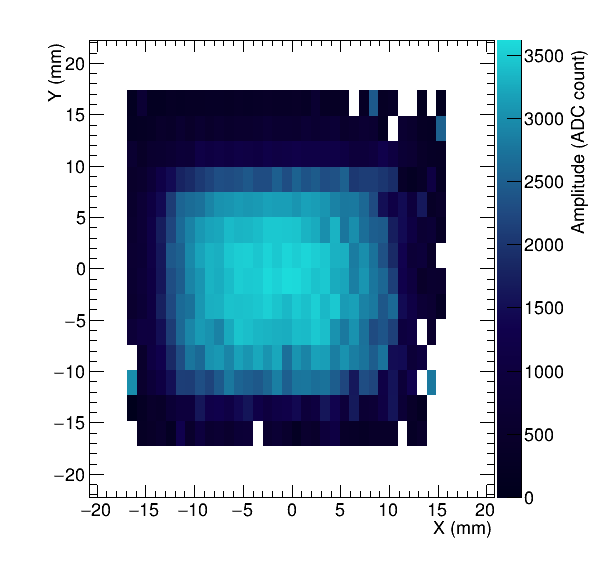
\includegraphics[width = 0.7\textwidth]{figures/upgrade/crystal_amp_map.pdf}
  \caption{Distribution of the signal amplitude of a single crystals as a function of the transverse inpact position for
    a 50 GeV electron beam. For alignment porpouses the events shown in the picture
    were acquired requiring only the coincidence between the \sixbysix and \threebythree scintillators.
    The crystal front face is a square with 22 mm sides, the area covered by the crystal is clearly visible in the amplitude
    profile as the light area at the center.}
  \label{fig:crystal_amp_map}
\end{figure}

\subsubsection{Amplitude and time reconstruction at the beam test}
The CAEN digitizer has 32 channels and for each event and channel acquires 1024 samples (one every 200 ns). The
digital conversion is performed by a 12-bit DAC, the dynamic range of the DAC is 1 V.
The channels are syncronized at a level better than 5 ps.
The samples were shipped to a commercial PC through the VME bus and an optical interface, the event
syncronization between the digitizer, hodoscopes and wire chamber data was performed by software running on the
acquisition PC.

The MCP signal is very fast, lasting 4 ns, its amplitude is estimated with a second order polinomial fit to the seven samples
around the maximum one while the time extracted with a constant fraction method to avoid amplitude walk effects.

The signal from the SiPM is readout through a NINO chip that provides both the time and amplitude measurements.
The signal time is extracted with a precision under 10 ps as the the time at which the signal pass a threshold that
can be configured. This method is very sensibile to the amplitude walk effect and the measured time is therefore
corrected during the analysis.

The amplitude and time of the APD signal are estimated with a template fit to the signal shape where the signal
amplitude and time of the maximum are free to float.
The template shape is build as the average of $1\times 10^5$ signals aligned using the time of the MCP signal
in the same event and scaled by the amplitude estimeted with the same approach used for the MCP signal.
A different template shape is constructed in this way
for each crystal. Two template examples are shown in Figure~\ref{fig:apd_templates} for channel with different  
shaping times. The template fit gives the best time performance for APD signals which has a smaller $dV/dt$ compared
to the MCP one.

\begin{figure}
  \centering
  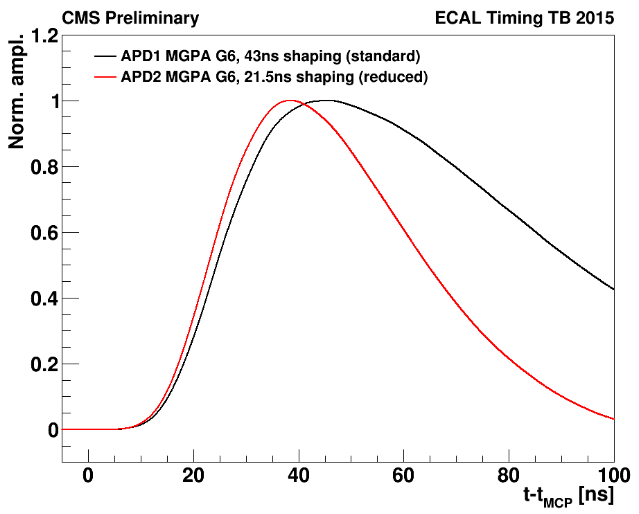
\includegraphics[width = 0.7\textwidth]{figures/upgrade/wf_shaping_times.png}
  \caption{APD signal average shape for 21.5 ns and 43 ns shaping times.}
  \label{fig:apd_templates}
\end{figure}

\subsubsection{Beam test results}
The resolution of the \PbWO crystals plus APDs system is extracted from 
the distribution of the time difference between the time measured by the MCP ($t_{MCP}$) and the crystal ($t_{APD}$)
hit by the electron.
A gaussian function is fit to the distribution and the standard deviation extracted from the fit is quoted as
the time resolution. The operation is performed at different energies and for two channels with different
amplifier shaping times. Only events in which the electron entered the crystal within 1.5 mm from the center of the
front face where selected. 

Figure~\ref{fig:results_treso} shows the results for the two different shaping times.
The resolution as a function of $A/\sigma_{n}$ is parametrized by the same Formula~\ref{eq:ecal_time_res} used in the
pre-installation test beam adjusting the constant term to take into account the known MCP resolution:
\[
  \sigma^2(t_{APD} - t_{MCP}) = \left( \frac{N\cdot\sigma_n}{A} \right)^2 + C^2 + C_{MCP}^2
\]
where $A$ and $\sigma_n$ are the average amplitude and noise of the APD signal at a given energy, $C_{MCP} = 25 ps$ is
the MCP time resolution and $N$, $C$ are the noise and constant term of the ECAL channel which are free to float in the fit.
As expected, for the same beam energy, the shorter 21.5 ns shaping has a larger amplitude than the 43 ns shaping one,
however in the fit data from both configurations are used.

The measured constant term is $27 \pm 1 ps$ close to the $20 \pm 4 ps$ value measured at the pre-installation test beam comparing the
time of two crystals inside the some electromagnetic shower.
The single channel noise at the test beam setup was found to be eight time as much the one measured in the current ECAL barrel
($A/\sigma_{noise} \sim 800$ for a 50 GeV electron or photon in ECAL), proving that a precision better than 50 ps could
be achieved for modetare energies of at least 25 GeV.

\begin{figure}[h!]
  \centering
  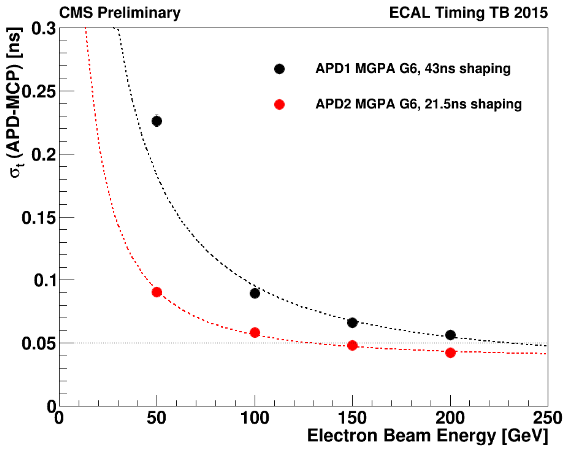
\includegraphics[width = 0.45\textwidth]{figures/upgrade/APD_t_res_vs_energy.png}
  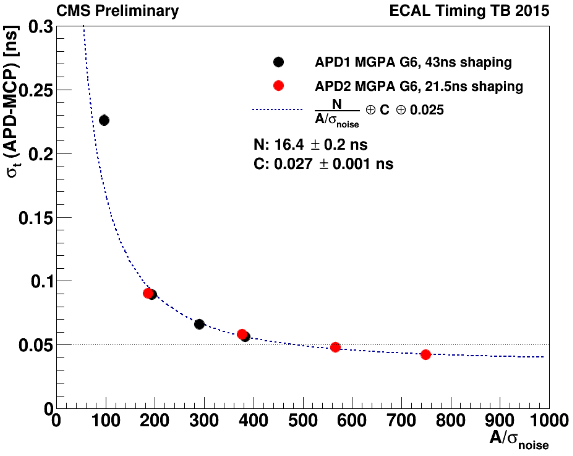
\includegraphics[width = 0.45\textwidth]{figures/upgrade/APD_t_res_vs_AoverN.png}
  \caption{Time resolution on $t_{APD}-t_{MCP}$ as a function of the beam energy (left)
    and the average signal $A/\sigma_n$ (right).
    In the left plot the lines are drawn to guide the eye while in the left plot the curve is the result of the
    fit described in the text.}
  \label{fig:results_treso}
\end{figure}

The impact of fluctuation in the light production depth on the time performance is estimated comparing the
time performance of the SiPM with that of the APDs. As illustrated in Figure~\ref{fig:light_collection_scheme}, 
the elctromagnatic shower propagates faster than the scintillation light in the crystal by a factor equal
to the \PbWO refractive index ($n=2.2$). The different propagation velocity can spoil the time resolution and the
effect is maximized when collecting the scintillation light on the front face since light produced later, deeper in
the crystal also travels a longer mimimum path to reach the photodetector on the front face than the one on the rear face.

\begin{figure}[h!]
  \centering
  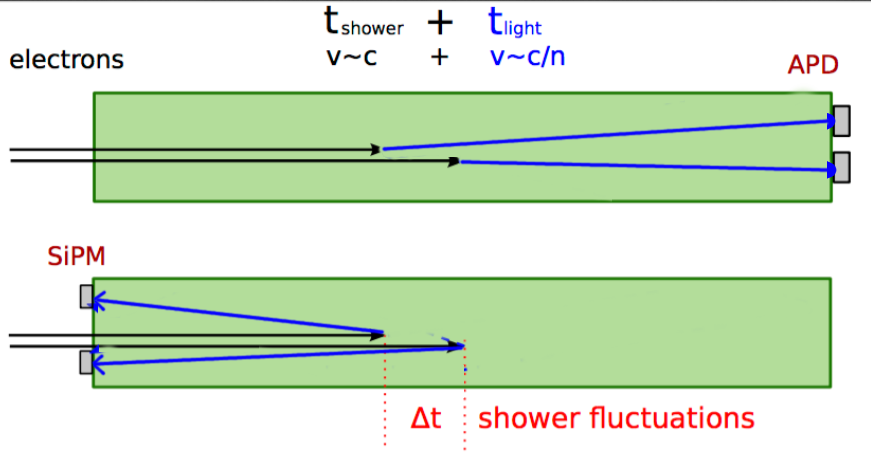
\includegraphics[width = .6\textwidth]{figures/upgrade/shower_fluct_cartoon.png}
  \caption{Illustration of light collection on the front and back face of the \PbWO crystal.}
  \label{fig:light_collection_scheme}
\end{figure}

The intrinsic time resolution of the SiPM arrays is estimeted comparing the time measured by the two different arrays using
the same procedure described for APD and MCP comparison. In this comparison shower depth fluctuations cancels since
are common to both SiPM arrays.
The result and the fit are shown in Figure~\ref{fig:sipm_tres},
the fitted time resolution constant term is 25 ps comparable to that of the APDs.
The time resolution is worse when comparing the time measured by one of the SiPM arrays to the one recorded by the MCP,
showing that fluctuation in the light emission depth impact the time resolution adding $\sim 80$ ps in quadrature regardless
of the shower energy which is clearly not affecting the APD performance.

\begin{figure}[h!]
  \centering
  \includegraphics[width = .7\textwidth]{figures/upgrade/sipm_50um_intrinsic.pdf}
  \caption{Front face light collection time performance. The times measured with the two SiPM arrays
    is compared to the MCP time (grey curves) and one to the other (red curve). SiPM time performance is comparable
    to the APDs one (red) but is affected by light emission fluctuations when comparing to an external
    reference (i.e. MCP).}
  \label{fig:sipm_tres}
\end{figure}

In 2016 a similar test was conducted with a prototype of the HL-LHC readout electronic installed in place of the
CR-RC amplification. The signal from the TIA amplifier was digitized with the same VME board used in 2015 and the
160 MHz sampling ADC is simulated at the analysis level by sampling the signal shape acquired at 5 GHz by the CAEN digitizer.
The beam test setup included also the same MCP and hodoscopes described~above. 

The event selection and time reconstruction is performed in the same way as for the 2015 beam test.
The results are reported in Figure~\ref{fig:tia_tres}: the time performance achieved by emulating the
160 MHz sampling is identical to the one obtained with 5 GHz sampling while at 80 MHz sampling the time resolution
depends on the sampling phase. ??

\begin{figure}[h!]
  \centering
  \includegraphics[width = 0.7\textwidth]{figures/upgrade/sampling_freq_res_comp.png}
  \caption{Time resolution performance of HL-LHC ECAL readout electronics for different sampling frequency.
    The baseline 160 MHz sampling frequency does not limit the time performance while the 80 MHz sampling
    performance depends on the phase between the electronics clock and the APD signal.}
  \label{fig:tia_tres}
\end{figure}


\clearpage\chapter{Conclusions}
\label{chapter:conclusions}

The research activity of my three years long Ph.D. activity was carried out within the
CMS experiment collaboration. The primary focus has been the search for BSM signatures in
diphoton events with data of proton-proton collisions at 13 TeV of center-of-mass energy collected by the CMS experiment.
The results obtained from the search for exotic spin-0 and spin-2 resonances improves the previous results
from LHC experiments and set limits on the production of RS graviton excluding resonances up to 2 to 4 TeV depending
on theory parameters.

An excellent photon energy resolution is required to achieved the best sensitivity to narrow resonances. Part
of my work was devoted to the energy calibration of the CMS ECAL, the crucial component for measurement involving
photons. The first energy calibration performed after the long LHC shutdown for the preparation of the 13 TeV run
restored the same energy resolution achieved during the 8 TeV operation. I optimized one of the
intercalibration methods which turned out to provide the best intercalibration precision among
the three methods used. The same method was further developed during 2016 to establish a monitoring of
the energy response evolution that combined with the laser monitoring system provides the stability needed
for precise measurement in the context of the Higgs boson physics in the diphoton final state.

Final states with photons will remain a powerful tool to explore the Higgs sector through precise
measurement of its properties and physics beyond the standard model also during the high luminosity phase
of LHC (HL-LHC). The instantaneous luminosity of the HL-LHC will pose severe challenges to the performances of
the physics analysis of CMS, due to the increased number of pileup events several observable (from diphoton
vertex reconstruction to b-tagging and isolation) will provide less discrimination power between signal
and background than they currently does.

CMS is planning a substantial upgrade of the detector for the HL-LHC phase including a new tracker system
with extended coverage, a high granularity sampling calorimeter for the endcaps, extended muons acceptance and
a Level-1 trigger system capable of recording events at 750 MHz (7.5 times the current rate).
The addition of time information to the event reconstruction has been also considered lately as a way to mitigate the
performance deterioration. From the simulation work presented in this document a clear benefit is brought
to the muon identification and the diphoton vertex reconstruction, other improvements have been demonstrated and were briefly
presented. All the studies underlines that only with time measurement for all charged particles it is possible
to reconstruct the time of the hard interaction and thus fully exploit the time-aware reconstruction combining
also the time measurement performed by the calorimeters. This requires the installation of a new
detector with a resolution of about 30~ps for charged particles with $p_T>0.7$ GeV. I took part in several beam
test aimed to establish the best technology for the implementation of such detector given the installation and operation
constrains of the future CMS detector. The LYSO crystal coupled to SiPM proved to be an already mature
technology with bout 30~ps time resolution on MIP suitable to be installed in the CMS barrel timing detector.
Regarding the calorimetry timing beam test results shows that the \PbWO plus APD sensor already installed in CMS
is capable of an excellent time resolution that with the future electronic will provide a precision of 20~ps
for electrons and photons with energy above $20$ GeV.


\backmatter
\bibliographystyle{unsrtnat}
\setcitestyle{numbers}
\bibliography{biblio}

\end{document}